\documentclass[12pt]{report}
\usepackage[utf8]{inputenc}
\usepackage[a4paper, margin=2.5cm]{geometry}
\usepackage{fancyhdr}
\usepackage[round]{natbib}
\usepackage{hyperref}
\usepackage{xcolor}
\usepackage{graphicx}
\usepackage[noend,ruled,vlined]{algorithm2e}
\usepackage{pdfpages}
\usepackage[acronym, nonumberlist]{glossaries}
\usepackage{minted}
\usepackage{subcaption}

\newcommand{\changefont}{%
    \bfseries\fontsize{8}{11}\selectfont
}

% Para checkmarks e xmarks
\usepackage{amssymb}% http://ctan.org/pkg/amssymb
\usepackage{pifont}% http://ctan.org/pkg/pifont
\newcommand{\cmark}{\ding{51}}%
\newcommand{\xmark}{\ding{53}}%

% Para tabelas
\usepackage{threeparttable}
\usepackage{array}
\usepackage{multirow}
\usepackage{booktabs}
\usepackage{pdflscape}
\usepackage{rotating}

\fancyhf{}
\cfoot{\thepage}
\renewcommand{\headrulewidth}{0pt}
\fancyhead[R]{\changefont \nouppercase \rightmark} %section
\pagestyle{fancy}

\def\CCBY{\CCaux{by}{CCBY.png}{CC BY}}

\def\CCaux#1#2#3{%
\noindent\includegraphics[width=0.2\textwidth]{img/#2}\\{\textbf{\textsf{#3}}}
\\\url{https://creativecommons.org/licenses/#1/4.0/}\\}

\renewcommand{\baselinestretch}{1.5}

% Defining extra colors
\definecolor{dark-blue}{cmyk}{1.0,1.0,0.0,0.1}
\definecolor{dark-green}{cmyk}{1.0,0,1.0,0.4}
\definecolor{dark-red}{cmyk}{0,1.0,1.0,0.3}
\definecolor{navy-blue}{cmyk}{1.0,1.0,0.0,0.1}
\definecolor{grey}{rgb}{0.6,0.6,0.6}
\definecolor{eng}{cmyk}{0.14,0.71,1,0.03}
\definecolor{um}{cmyk}{0.25,1.00,1.00,0.22}
\definecolor{lightGray}{gray}{0.92}

\hypersetup{
%    bookmarks=true,						% show bookmarks bar?
	bookmarksnumbered=true,
	plainpages=false,					 	
    unicode=true,					 		% non-Latin characters in Acrobat’s bookmarks
    pdffitwindow=true,						% window fit to page when opened
    %pdfstartview={FitW},					% fits the width of the page to the window
    %pdftitle={My title},					% title
    pdfauthor={Rui Oliveira},		            % author
    %pdfsubject={Subject},					% subject of the document
    pdfcreator={Rui Oliveira},		            % creator of the document
    pdfproducer={Rui Oliveira},		        % producer of the document
    %pdfkeywords={keyword1} {key2} {key3},	% list of keywords
    %pdfnewwindow=true,						% links in new window
    colorlinks=true,						% false: boxed links; true: colored links
    linkcolor=dark-blue,					% color of internal links
    citecolor=dark-green,					% color of links to bibliography
    filecolor=magenta,						% color of file links
    urlcolor=navy-blue						% color of external links
}

\makeglossaries
\loadglsentries{glossaries}

\begin{document}

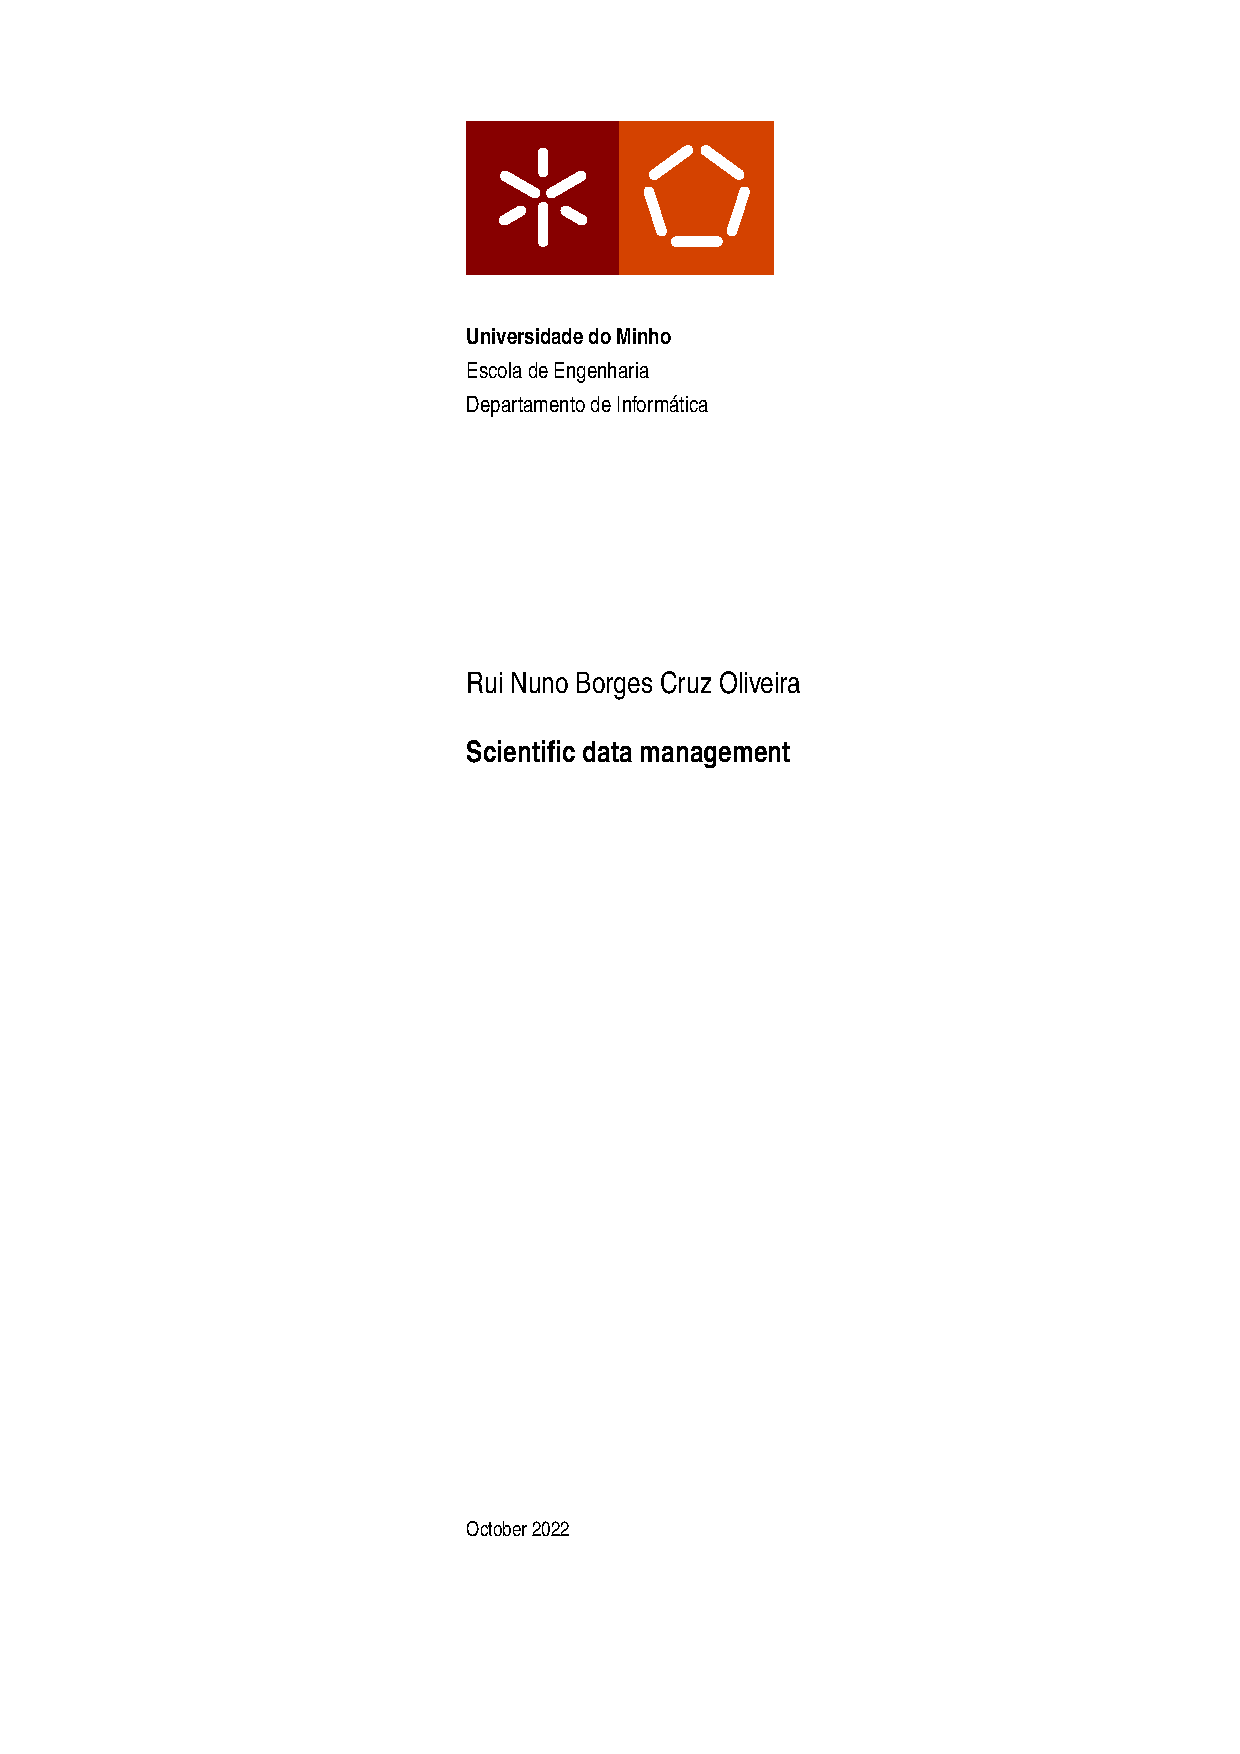
\includepdf{cover/frontcover.pdf}
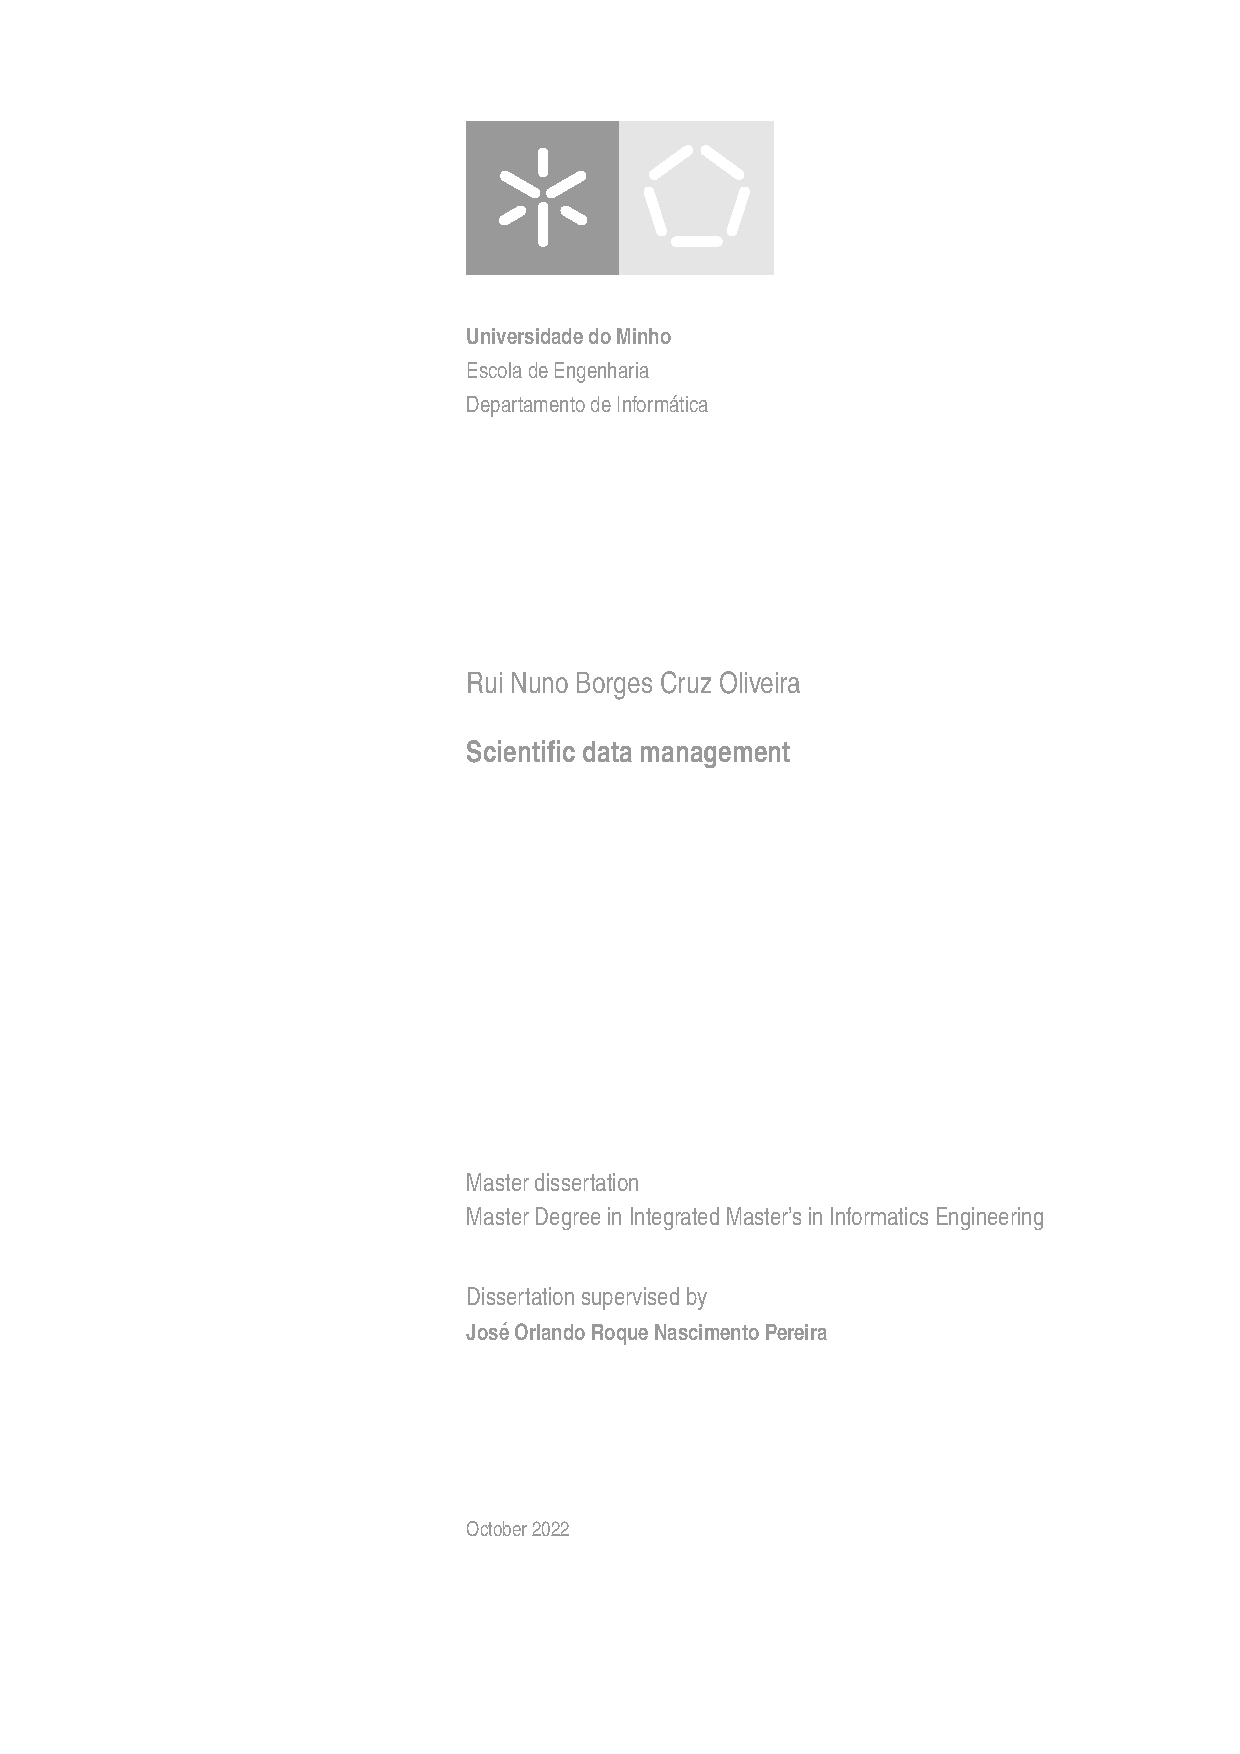
\includepdf{cover/backcover.pdf}

\pagenumbering{roman}
\setcounter{page}{1}

\chapter*{Copyright and Terms of Use for Third Party Work}

    This dissertation reports on academic work that can be used by third parties as long as the internationally accepted standards and good practices are respected concerning copyright and related rights.
\vskip 1em
\noindent This work can thereafter be used under the terms established in the license below.
\vskip 1em
\noindent Readers needing authorisation conditions not provided for in the indicated licensing should contact the author through the RepositóriUM of the University of Minho.

\vskip 1em
\noindent \textbf{\textit{License granted to users of this work}}
\vskip 1em

\CCBY

\chapter*{Acknowledgments}

    Throughout the writing of this dissertation, I have received a great deal of support and assistance.

I would like to express my sincere gratitude to my supervisor, Professor José Orlando Pereira. Without his guidance and assistance throughout the process, the outcome of this dissertation would not be the same.

While doing this work, I had a Research Grant from INESC TEC funded by National Funds, so I also want to thank FCT (Fundação Portuguesa para a Ciência e Tecnologia) and INESC TEC. In particular, a word of thanks to Susana Barbosa, researcher at INESC TEC and one of the coordinators of the SAIL Project, her assistance was invaluable.

To my family, I would like to express my deep gratitude for always being there and for always supporting me throughout my academic journey, providing everything I needed. Certainly, without them, these last five years would not have been possible.

A special thanks to my friends, in particular those who have lived this experience closely, they have made all the effort rewarding. These five years will always be remembered for the beautiful stories we lived together.

The last word of appreciation goes to my dear Lídia, for her unconditional support at all times. I am thankful that she appeared on this journey and never let me down. Thank you for always encouraging me to be the best version of myself.


\chapter*{Statement of Integrity}

    I hereby declare having conducted this academic work with integrity.
\vskip 1em\noindent
I confirm that I have not used plagiarism or any form of undue use of information or falsification of results along the process leading to its elaboration. 
\vskip 1em\noindent
I further declare that I have fully acknowledged the Code of Ethical Conduct of the University of Minho.

\chapter*{Abstract}

    Universally, it is known that data is constantly changing, new concepts emerge and ways to represent them, and sometimes many of these concepts become deprecated. In the context of scientific research, data management is no exception, as it becomes more challenging to deal with the growing volume of data and with the complexity of the surrounding techniques. Furthermore, it is common in companies, as well as in scientific research, a huge dependence on those who are responsible for the management of all the information, leading to the possibility that team changes are not as efficient as one would expect. It is therefore crucial to analyse, organise and document data.
    
There are several techniques developed over the last years to deal with this problem, and the main focus of this dissertation is to adapt and apply the most appealing in the scrutiny of the currently known systems to handle the management of scientific data. These systems will be compared considering the following criteria: architecture, interoperability, metadata, usability and security. Finally, after adapting one of the solutions, a performance evaluation will be required in order to extrapolate its functioning in a real-world context.

\paragraph{Keywords} Scientific data management, research, CKAN, EUDAT
    
\chapter*{Resumo}

    Universalmente, sabe-se que os dados estão em constante mudança, surgem novos conceitos e formas de os representar, e por vezes muitos destes conceitos são depreciados. No contexto da investigação científica, a gestão de dados não é excepção, pois torna-se mais desafiante lidar com o volume crescente de dados e com a complexidade das técnicas que os rodeiam. Além disso, é comum nas empresas, bem como na investigação científica, uma enorme dependência daqueles que são responsáveis pela gestão de toda a informação, levando à possibilidade de as mudanças de equipa não serem tão eficientes como seria de esperar. É, por conseguinte, crucial analisar, organizar e documentar os dados.
    
Há várias técnicas desenvolvidas nos últimos anos para lidar com este problema, e o foco principal desta dissertação é adaptar e aplicar o mais apelativo na análise dos sistemas actualmente conhecidos para lidar com a gestão de dados científicos. Estes sistemas serão comparados considerando os seguintes critérios: arquitectura, interoperabilidade, metadados, usabilidade e segurança. Finalmente, após a adaptação de uma das soluções, será necessária uma avaliação de desempenho a fim de extrapolar o seu funcionamento num contexto do mundo real.

\paragraph{Palavras-chave} Gestão de dados científicos, investigação, CKAN, EUDAT
    
\cleardoublepage
\tableofcontents

\cleardoublepage
\addcontentsline{toc}{chapter}{\listfigurename}
\listoffigures
	
\cleardoublepage
\addcontentsline{toc}{chapter}{\listtablename}
\listoftables

\cleardoublepage
\printglossaries
\addcontentsline{toc}{chapter}{Glossary}

\cleardoublepage
\pagenumbering{arabic}
\setcounter{page}{1}
    
\chapter{Introduction}

    \label{ref:chapter_1}

Collaboration plays a crucial role in scientific innovation because the problems faced are of such complexity that no single individual or collective has all the relevant information, knowledge or resources \citep{loshin}. Scientific research depends on an efficient and organised means of technological communication so that research can be exploited and improved to its full potential \citep{fair}. This requires special consideration of data resulting from investigation, regardless of whether they are large or small.
  
The better an organisation understands its data, the better it can use it and consequently share it with the scientific community and allow the same data to be repeated and improved. Hence, we can effectively say that the speed at which science evolves today depends on how and whether data sharing is done \citep{10}.

While at first glance it may seem obvious that all research collectives would like to make global collaboration a widespread practice, since we are talking about the evolution of science, this is not necessarily the case \citep{tenopir}. In essence, science is also an industry, and the investment of time and money is something that has to be put on the table and made as efficient as possible \citep{3}. As such, instruments to implement information sharing have to meet certain criteria for research institutions to invest in them.

    \section{Problem}
    	Every year new topics appear on the agenda of researchers and scientists, and all over the world research teams dedicate themselves publicly or privately to the most varied problems. The same research may be carried out by different organisations, which, with different resources and ways of working, produce huge volumes of data and make subjective analyses of them. 

This reality led to the emergence of the problem of how the management of the work produced should be carried out and, with this, generated the question of the need for mechanisms and systems that allow the way of working to be universalised \citep{9}. Thus, the issue better known as scientific data management arose.

There are several known solutions to this problem, and the systems responsible for this management may or may not have research data as a priority, the important thing is to understand if the functionalities they support are the most useful in solving the problem. Basically, the choice of a solution depends on the particularities of the research of the promoting entities, so before choosing a system, it is necessary to define the aspects to be evaluated \citep{dong}.
  
Specifically, this dissertation will take as a case study the \gls{sail} project carried out by \gls{inesctec} on board the School-Ship Sagres, the object of study of the project being atmospheric electricity and climate change, and aims to develop a scientific observation platform to collect data on the ocean and atmosphere \citep{2}. This will allow us to have a concrete idea of what a system should provide for a specific research case.
 
Despite the significant growth of existing solutions in the market, most scientific institutions, especially those linked to universities, still have their own data repository. This is due to the fact that performance capacity is something to be considered, since unlimited fast access at any time requires a certain amount of computing power, particularly if there is the premise of growing the repository and with it the accesses to it \citep{6}. Therefore, it would be interesting to understand how a solution can be integrated into supercomputing and big data infrastructures, more specifically, with the help of the \gls{macc}, which is developing the installation of the new Portuguese supercomputer Deucalion at AvePark, in Caldas das Taipas, Guimarães. In this case, we have to consider that the data stored in the system to be developed should be accessible through compute servers. For example, a File System (FS) such as Lustre (an open source parallel FS that supports many requirements of \gls{hpc} simulation environments) should be used for its data storage in a seamless and transparent manner.

    
    \section{Objectives}
        Firstly, the objective of this dissertation is to understand how some of the existing software systems and international cooperation networks work to solve the problem mentioned, and, more than understanding how they work, to understand, concretely, what they offer.

With this in mind, once the evaluation is done, the objective is to adapt and apply an existing system so that it can correspond in the most efficient way to scientific research, with special attention to the particularities promoted by the case study of this dissertation, the \gls{sail} project.

Finally, it will be necessary to evaluate the performance of the developed system, important to understand how it might behave in a real context. For this, ideally we would use \gls{macc}, which, by promoting and supporting open scientific initiatives on advanced computing, data science and visualisation, could play a fundamental role in this project in terms of understanding how to adopt a system to real scenarios of considerable computing power. However, in the event that it is not possible for us to use \gls{macc}'s resources, since the installation of Deucalion may still take some time, we will use the resources of \gls{inesctec}, which, although it does not allow us to have the understanding that \gls{macc} would make possible, serves to give us a notion of how the system we develop works and will allow us to extrapolate its use, after the writing of this dissertation, in an infrastructure like \gls{macc}.
        
    \section{Structure}
        This dissertation is divided into several chapters, and the first provides the context, problem and general objectives of the work. Next, Chapter \ref{ref:chapter_2} allows us to review the state of the art, with the background and related work. In Chapters \ref{ref:chapter_3} and \ref{ref:chapter_4} we expose all the details of the implemented solution, how to use it and the results of the performance evaluation. Finally, the Chapter \ref{ref:chapter_5} presents the conclusions drawn and guidelines for future work.

\chapter{State of the Art}

    \label{ref:chapter_2}

This chapter introduces the state of the art of this dissertation, which is divided between two sections: background and related work.

Firstly, we provide an overview of the use of \gls{dms}s, as well as their different models and approaches. Furthermore, we provide a contextualisation regarding the case study under consideration, describing its particularities. Finally, we discuss the different criteria for evaluating a \gls{sdms} as a response to the problem of scientific data management.

Secondly, we thoroughly analyse each of the three systems considered in this work, that is, \textit{\gls{ckan}} \citep{ckn}, \textit{\gls{eudat}} \citep{eud} and \textit{Magda} \citep{mgd}, and subsequently we perform an evaluation and comparison between them to understand which is best suited for managing scientific data, with special attention to our case study.
    
    \section{Background}
    
        \label{sec:background}

\subsection{DMS}
  
\gls{dms} provides a self-service environment for users to access, define, and manipulate data. The powerful tools in such a system use metadata management to automate data organisation, to show relationships between data, and some even include functionality for government, business, or scientific data \citep{7}.

Databases are the most common platform for data management, but file systems or cloud object storage services are also used, which generally offer greater flexibility over databases since they organize data in a less structured way. 
  
\gls{dms}s have evolved and now present several options regarding the data model. A data model is an abstract model that organises data elements, documents how data is stored and retrieved and designs the necessary response to information system requirements. The main existing models are as follows:
  
\begin{itemize}
    \item Hierarchical data model, each component has a child/parent relationship with another component;
    \item Network data model, each component can have multiple relationships;
    \item Relational data model, each component has attributes that are linked to their identities through a table structure.
\end{itemize}
  
Other data models include graph database, relation-entity, and object-oriented.
  
This dissertation will focus on \gls{sdms}s, which aim to increase the productivity of any research without neglecting any sharing and collaboration efforts. \gls{sdms} is a better approach to handle unstructured data, which includes images, PDF files, spreadsheets, geographic coordinates, and other data formats resulting from an investigation. 

\subsection{\label{tab:sail_project}SAIL Project}

The case study focus on measuring the electric field of the atmosphere over the ocean and monitoring gamma, solar and cosmic radiation or \gls{gnss} signals, as well as taking into account other aspects such as temperature and pH. That being said, we can see that the study has a wide diversity of data, and it is also important to consider the fact that this campaign collected data every second, with hourly records for 371 days.
  
We needed to understand what data would need to be considered and how they are organised in order to adapt the system we intended to develop. Therefore, in order to find an answer to this point, we tried to meet with the project's research team, and we were able to meet with one of the members who informed us about the campaign data we need to work with:

  
\begin{itemize}
    \item \gls{gnss} data, which refers to a constellation of satellites providing signals from space that transmit positioning and timing data to \gls{gnss} receivers. \gls{gnss} data can be represented in different formats -- binary, RAWIMUX, and \gls{nmea} -- with \gls{nmea} being the one to pay particular attention to  when testing the volume of data;
    \item Atmospheric data, specifically electric field (E1 and E2), gamma radiation (GA), visibility (VI) and radiation (inSL and outSL), which constitute a smaller sample compared to the first type, referring to 30/60 days. These data are more interesting and easier to work with, since they were previously processed and subjected to quality control procedures.
\end{itemize}

In order to organise the data, a conventional nomenclature was adopted, consisting of: activity type + infix data group + infix measured parameter. Regarding the \gls{gnss} data we will explore, these are divided into 2 groups: ship data (SHIP) and sensor data (SD), and atmospheric data are in the pre-processed data (PD) group. Therefore, the following is the nomenclature that will be used in the datasets and system files:

\begin{itemize}
    \item GNNS - SAIL\_SHIP\_GNSS\_*
    \item GNNS \gls{nmea} standard - SAIL\_SD\_GNSS\_NMEA\_*
    \item Atmospheric fields - SAIL\_PD\_E1\_*, SAIL\_PD\_E2\_*, SAIL\_PD\_GA\_*, SAIL\_PD\_VI\_*, SAIL\_PD\_inSL\_*, SAIL\_PD\_outSL\_*
\end{itemize}

The * above denotes two possibilities -- yyyymmddd for compressed files or yyyymmddd\_hh for files -- where yyyy is the year, mm is the month, dd is the day and hh is the hour. 

There were two antennas collecting information from the Sagres ship and each compressed file includes information collected per day by those antennas. Each compressed file includes files with data associated with each hour of the day, i.e. a total of 48 files per day.
  
\newpage  
  
\subsection{Key Criteria for SDMSs}
  
Key criteria are defined by three dimensions: architecture, interoperability \& metadata, and usability \& security.
    
\begin{table}[!h]
    \centering
    \caption{Key criteria by dimension}
    \begin{tabular}{|c|c|c|} 
        \hline
        Architecture                & Interoperability \& metadata    & Usability \& security      \\ 
        \hline
        Installation and deployment & \gls{api}s                            & Popularity                 \\
        Open source                 & Harvesting protocols            & Advanced search            \\
        Storage replication         & Standard schemas                & Geospatial tools           \\
        Storage location            & Validation                      & Authorised authentication  \\
        Customisation               & Federation                      & Curation workflow          \\ 
        \cline{1-1}\cline{3-3}
        \multicolumn{1}{l|}{}       & Digital Object Identifier (DOI) & \multicolumn{1}{l}{}       \\
        \cline{2-2}
    \end{tabular}
\end{table}
    
\subsubsection{Architecture}
	
The installation and setup of any system should be as easy and flexible as possible. This work can usually be done through some repository of the institution that owns the platform or by outsourcing an external service (\textit{Docker}, for example). Moreover, free access to the source code allows a better study and, consequently, understanding of the developed software. Furthermore, the fact that the code is not open source exposes the possibility that the platform's support is not done indefinitely and depends on third parties \citep{1}.
	
In a specific case for any \gls{dms}, if its database fails for a moment, it will not be a problem if we consider database replication, otherwise we may lose all the information. As such, storage replication will also be an important aspect to consider.
	
Finally, other interesting aspects to consider are the location where the data is kept (remotely or locally), and the ability of the system to be customised as well as extended. The latter allows the community to develop scientific data management solutions that are not restricted by the existing functionalities.
	    
\subsubsection{Interoperability and metadata}
    
On the one hand, the existence of \gls{api}s in a scientific data management solution, allows its integration into external systems, which grants greater visibility and subsequent improvement of its content. On the other hand, metadata interoperability can be facilitated through compliance with standard protocols for harvesting metadata, such as the Open Archives Initiative Protocol for Metadata Harvesting (OAI-PMH) \citep{1}, with harvesting metadata referring to the automated collection of metadata description from several places to generate useful aggregations of their information. 
    
Along with protocols such as OAI-PMH, metadata standardisation can be useful, because if everyone uses different standards it can be very difficult to compare and analyse data \citep{7}. Moreover, to ensure that the data to be analysed is correct, data validation is advantageous when creating any dataset.
    
Federation with a web service should be possible, since the creation of a federated network of data portals that share and disseminate information between each other is very useful, as it provides the interoperability, consistency, and access controls needed to enhance the cooperation and security policies between the different research centers across multiple networks.    
    
From a long-term perspective, assigning a persistent unique identifier to the resources that are stored, like Digital Object Identifier (DOI), is also very important, as it persists with each resource forever, even if its location or form of storage changes over time, which also makes it easier to cite resources that could be extremely useful to any researcher.
    
Finally, the resources available in the system may be used freely or not, since any user holding a given dataset has the right to protect the use of its content. Therefore, the platform must guarantee the possibility of granting a licence to any data.
    
\subsubsection{Usability and security}
    
Lastly, there are also a few more criteria in a more general overview that also deserve attention. First, as any solution to any problem on the market is also evaluated by its popularity, \gls{sdms}s are no exception, as it is natural to assume that greater popularity leads to greater use and validation (or not) of the product. In addition, it enhances the diffusion of the solution and increases the size of the community, which allows for an improvement in knowledge and consequent usability for the system in question.

Another relevant factor to usability is its search, the aim being as intuitive and intelligent as possible. More than allowing a simple search, it is important to consider advanced search features, as it offers a greater number of tools for any researcher to find what they want more easily. Likewise, advanced geospatial features can be advantageous to use in the context of scientific investigations.
    
Some security policies can be offered to organisations that use data management solutions, one of which is authorised authentication, in other words, it is possible that these same organisations control who can carry out actions on their resources. For example, authorisation systems can manage who can register/delete new users, or who can edit/create/delete datasets.
    
Usually, researchers are not experts in data management, therefore, they need intuitive and efficient tools to produce the intended results without the need for complex learning about the functioning of an effective solution to the problem of managing scientific data. Not to mention that the available workflow has to be viable both in the immediate and long term to scientific research, that is, curation workflow.  
    
In short, any solution that is easy and safe to use is closer to being adopted in the daily work of an investigator.
            
    \section{Related Work}
    
        \subsection{\textit{CKAN}}
  
\textit{\gls{ckan}} is an open-source data management solution whose main objective is to allow the creation, access, and dissemination of knowledge through tools for the use and reuse, publication, search and share of information. Generally, it is implemented by organisations and is used by several national governments to manage their data, but it can also be used by companies, research institutions, or even individuals. Currently, \textit{\gls{ckan}'s} design demonstrates a versatile range of options, and can be used as a catalog, repository, datastore, or as a combination of all three \citep{5}.
  
\subsubsection{Architecture}
  
\textit{\gls{ckan}} follows the classic \textit{Model View Controller (MVC)} pattern. There is a clear distinction between the various layers, where the data representation and client interaction, i.e. the View, are separated from the methods that interact with the databases, i.e. the Model, with the Controller mediating between the two through the changes that the user interacting with the system wants. This architecture is shown in and the Figure \ref{fig:ckan_arch}.
  
\begin{figure}[h!]
    \centering
    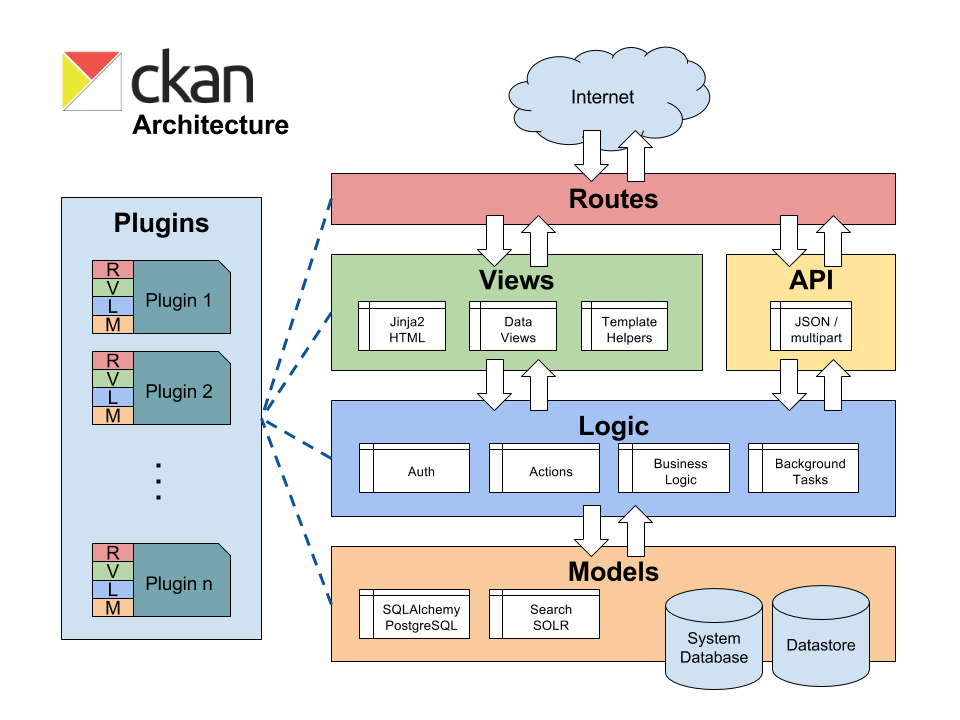
\includegraphics[width=0.9\textwidth]{img/state_of_the_art/architecture_ckan.png}
    \caption{\textit{\gls{ckan}} Code Architecture (http://docs.ckan.org/en/2.9/contributing/architecture.html)}
    \label{fig:ckan_arch}
\end{figure}
    
\textit{\gls{ckan}} is highly customisable and encourages the extension of content to the code base to adapt the system to different needs. The community and the \textit{\gls{ckan}} development team already have a vast list of extensions available.
  
\subsubsection{Installation}
  
The best option for \textit{\gls{ckan}'s} installation, which is currently in version 2.9 (version by which the evaluation of this platform will be guided), depends on the intended use of it. According to the documentation that the system provides, there are three ways to install it: 
  
\begin{itemize}
  \item Install from an operating system package;
  \item Install from source;
  \item Install from \textit{Docker Compose}, a tool for defining and running multi-container \textit{Docker} applications;
\end{itemize}
  
Installing from the package is the fastest and easiest way to get \textit{\gls{ckan}}, as it requires either the 18.04 64-bit or 20.04 64-bit version of Ubuntu. It is still necessary to install \textit{Solr} for the research tools and \textit{PostgreSQL} for the database. Moreover, this system is primarily written in \textit{Python}.
  
When the installation is well completed, two web applications will be running, \textit{\gls{ckan}} itself and the \textit{Datapusher}, a distinct service for automatically importing data to \textit{\gls{ckan}'s} \textit{DataStore} extension.
  
\subsubsection{Datasets, Role management and Authorisation}
  
With \textit{\gls{ckan}}, data is published in units called datasets, which contain two things: information relating to the data, in other words, metadata, and resources that contain the data, which can be stored as relational database entries or separate files (XML files, images or linked data in RDF format, for example).
  
Unlike other cloud services, \textit{\gls{ckan}} does not use a distributed data storage, since multi-user concurrency is not a major requirement in the way this software handles information. Instead, data integrity is generally favoured by data publishers to avoid data conflicts. Hence, \textit{\gls{ckan}}'s team decided to implement a central data store to meet their needs \citep{8}.
  
Typically, each dataset belongs to an organisation and each \textit{\gls{ckan}} instance can have numerous organisations. Considering, for example, the case of a scientific investigation that is being carried out by a research center that is using \textit{\gls{ckan}}, there may be different departments publishing data. In this case, each organisation can define its way of working and specific authorisations, providing tools to manage its data ingestion process. Thus, the platform becomes very versatile and there is no requirement for centralised management.
  
Within each organisation, there can be different levels of access, where admins can add users and specify the level of access for each one.
  
Despite the above, it is also possible to configure \textit{\gls{ckan}} with the objective that the datasets do not belong to any organisation, which opens up the possibility of a wiki-like \textit{DataHub}.
  
\subsubsection{Metadata}
  
By default, \textit{\gls{ckan}} offers the following basic set of metadata:

\begin{itemize}
  \item Title;
  \item ID;
  \item Groups;
  \item Description;
  \item Revision history;
  \item License;
  \item Tags;
  \item Formats;
  \item \gls{api} key.
\end{itemize}
  
It also allows other attributes, such as location data through the geographic feature or customised information relevant to the publisher or dataset. Although the \textit{\gls{ckan}} metadata does not follow any standard schema, the system, through the above-mentioned customisation, grants the inclusion of arbitrary key/value pairs, which can only be represented by strings \citep{1}.
  
\subsubsection{\textit{FileStore} and \textit{DataStore}}

\textit{\gls{ckan}'s} \textit{FileStore} allows users to upload files, which by default are stored locally on the server, so that \textit{\gls{ckan}} has more control over the files and manages access to them. However, some extensions allow the user to save files remotely, such as on \textit{Amazon S3} \citep{5}. Presently, only one storage location can be used.
  
The \textit{DataStore} extension provides a database to store structured data of \textit{\gls{ckan}} resources, and data can be extracted from files and saved in the \textit{DataStore}, whether initially in the \textit{FileStore} or external links. The upload work of both possible resource sources is from \textit{Datapusher}.
  
Therefore, there are two distinct ways of storing \textit{\gls{ckan}} resources. On the one hand, there is the \textit{FileStore} which provides a storage of files where access or filtering to specific parts is not possible. On the other hand, the \textit{DataStore} is like a database where accessing and filtering data elements is possible. For example, a file of the CSV type, in \textit{FileStore} would be stored as a whole and to access its content would be necessary a download, while in \textit{DataStore} it would be possible to access each line of the content of a CSV spreadsheet individually via an \gls{api}, as well as filtering content. Although \textit{\gls{ckan}} does not support data replication, it is possible to say that a partial replication of certain datasets can often occur under the simultaneous use of these two storage components.
  
\subsubsection{Interoperability}
  
Through its \gls{api}s, this system offers tools for developers who want to interact with \textit{\gls{ckan}} sites or their data. In addition to the \textit{\gls{ckan}} Action \gls{api}, an RPC-style \gls{api} that exposes the core functionalities of a \textit{\gls{ckan}} website to any external code, \textit{FileStore}, and \textit{DataStore} have their \gls{api}s. 
  
Despite the interoperability that allows via \gls{api}s, \textit{\gls{ckan}} fails to support, by default, compliance with standard protocols used by the scientific community such as the OAI-PMH. Furthermore, metadata records do not follow any specific schema, despite allowing the use of an extension that exposes and consumes metadata using Resource Description Framework (RDF) documents serialized using Data Catalog Vocabulary (DCAT), which is an RDF vocabulary developed to facilitate the interoperability between data catalogs \citep{4, 5}. Thus, \textit{\gls{ckan}} makes it possible to expose and consume metadata from other data catalogs with standards schemas, but at no point does it include their validation, which in this case is done by the entities that originate the data.
 
This system can be used to create a federated network of data portals that share and manage data with each other. This is achieved through the \textit{\gls{ckan}} harvesting extension, and it is even possible to federate data from \textit{non-\gls{ckan}} catalogs with the aforementioned DCAT extension.
  
\subsubsection{Search, preview and visualization tools}
  
\textit{\gls{ckan}} provides a search interface similar to \textit{Google}, allowing search by word, delimited or not by quotation marks. Users can easily get a list of available datasets and perform searches on them. There are several search options, which can all be performed via \gls{api}:
  
\begin{itemize}
  \item Search on all dataset attributes;
  \item Full-text search;
  \item Fuzzy-matching, option to find terms close to the one entered instead of exact terms;
  \item Faceted search, in other words, searching through specific fields, such as tags.
\end{itemize}
  
This platform can automatically preview some data types and extend an interactive analysis before downloading. The main features of content visualization include graphics, tables, maps (via advanced geospatial features), or images, and it is also possible to create new forms of preview for other types of data through extensions.
  
\subsection{\textit{Magda}}
  
\textit{Magda} is an open-source data catalog system that provides a single space for an organisation's data to be stored, cataloged, searched, and enriched, whether large datasets or small files. This system is designed around the concept of federation and with the flexibility to be used as a catalog of big data in a data lake, an easily searchable repository for small data files, an aggregator of data from multiple external sources, or all in one.
  
\subsubsection{Architecture}
  
One of \textit{Magda's} main characteristics is its architecture, which is presented in a diagram in Figure \ref{fig:magda_arch} and consists of an extensible set of micro services that are distributed as \textit{Docker} containers, in the sense that new services can be added allowing organisations to go beyond the standard system. Any extension to collect data or enrich metadata can be written in any language and added/removed without significant changes to the operation of the core system. The architecture of \textit{Magda} is presented in a diagram in Figure \ref{fig:magda_arch}.
  
The use of \textit{Kubernetes}, for orchestrating \textit{Docker} containers, and \textit{Helm}, which helps manage \textit{Kubernetes} applications, means that the configuration of a customisable \textit{Magda} instance can be stored and tracked as plain text, and instances with identical configuration can be replicated quickly.
  
  
\begin{figure}[!h]
    \centering
    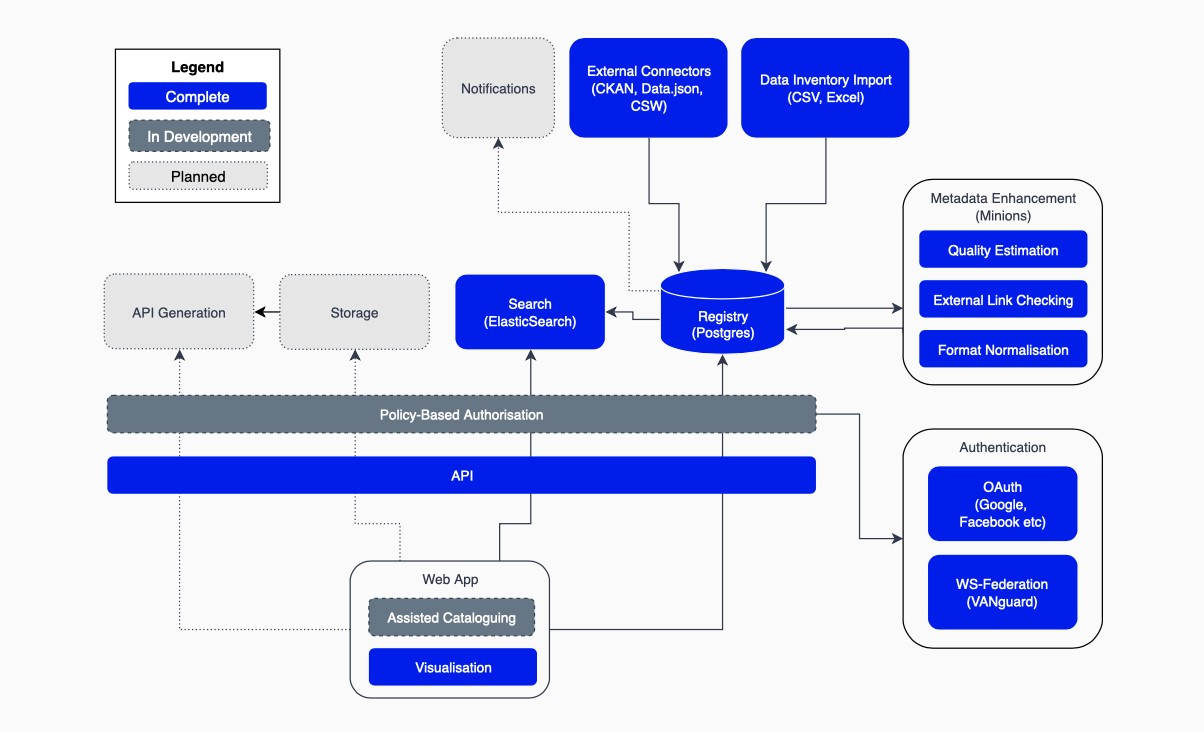
\includegraphics[width=1\textwidth]{img/state_of_the_art/architecture_magda.jpg}
    \caption{\textit{Magda} Architecture (https://magda.io/)}
    \label{fig:magda_arch}
\end{figure}  
  
\newpage  
  
\subsubsection{Installation}
  
\textit{Magda} can be installed in two ways, with the one chosen depending on the priorities of the user or organization:
  
\begin{itemize}
    \item Install from source;
    \item Install from \textit{Terraform}, a tool that provides a workflow for managing cloud services as \textit{Google Cloud}, or via another local or cloud environment.
\end{itemize}

Using \textit{Kubernetes} and \textit{Helm} enables simple installation and minimal system downtime. Configuration via pre-built images, i.e. from the second option in the list above, is simple in a setup as an open data search engine. However, using other features like adding datasets or the admin UI. setup is not so simple and \textit{Kubernetes} skills are usually required.
    
\textit{Magda} is currently under development, with their team looking to make the open source side more robust and adding new features to their implementations, which at the moment are not fully documented or require specific configurations to work.
    
\subsubsection{Authorisation and authentication}
  
At the moment a customisable authorisation system based on Open Policy Agent is being integrated, which will allow:
  
\begin{itemize}
  \item Restricting datasets based on the establishment of access control frameworks (through roles, for example) or policies specified by the organization;
  \item Control user access to content when searching for it;
  \item Federated authorisation.
  \end{itemize}
  
The latter not only allows data to be collected from external sources but also allows to mimic the same authorisations policies.
  
\textit{Magda's} authentication system, which is based on \textit{PassportJS}, an authentication middleware for \textit{NodeJS}, integrates a wide range of providers, such as \textit{Google}, \textit{Facebook}, or even the aforementioned \textit{\gls{ckan}}. In addition, it is also possible to develop authentication plugins to customise this process.
  
\subsubsection{\textit{Registry}}
  
\textit{Magda} works on the basis of a \textit{Registry}, an opinionless datastore built on top of \textit{PostgreSQL}, which stores records as a set of JSON documents called aspects. A dataset is represented as a record with several aspects - basic records containing the name or description, for example, or more complex ones like the quality or license of the data. Similarly, the actual data files or the URLs that link to them are also worked out as records, with their own sets of aspects. 

Aspects can be declared dynamically by other services through a call with name, description, and JSON schema. This allows the user to save extra information by declaring new aspects. Also, since the system is opinionless, it is possible to create new entities in the system that connect to each other.
  
\subsubsection{Metadata and \textit{Minions}}
  
The default metadata format used natively is the aspects system. \textit{Magda} has an unopinionated central metadata store and therefore can provide most metadata schemas but none as standard, i.e. it supports partial standardisation.
  
\textit{Magda} is ready to automatically enhance metadata without ever needing the data to be transmitted to a \textit{Magda} server. The process of adding datasets for those that are cataloged directly is able to derive data from the files directly in the user's internet browser. 
  
A \textit{Minion} is a service that observes new records or changes to existing ones, performs some operation and writes the result back to the \textit{Registry}. There are several aspects that are written by various \textit{Minions}, such as the quality aspect that contains content evaluations from different sources, which are averaged out and used by search. For both internal or external dataset, the \textit{Minions} framework is ready to act.
  
The framework for enhancement can be extended so that the user/organisation can build its enhancement process using any language that can be deployed as a \textit{Docker} container.
  
\subsubsection{Interoperability and \textit{Connectors}}
  
\textit{Magda} is designed with the ability to pull data from external sources into an easily searchable catalog in which all datasets are all one entity that supports all the operations available in the others, regardless of where they come from. However, it does not use any harvesting protocol such as OAI-PMH.
  
For the data collection process there are so-called \textit{Connectors}, \textit{Docker-based} micro services invoked as jobs, which go to external data sources and copy their metadata to the \textit{Registry}. Thus, the metadata can be searched and have other aspects attached to it. 
  
This system can accept metadata from its own cataloging process, and there are Excel or CSV-based data inventories and metadata \gls{api}s such as those from \textit{\gls{ckan}} or from its own REST \gls{api}. Moreover, the data here is combined into a single search index with history tracking and notifications when metadata records change.

\subsubsection{Search, preview and visualisation tools of data}
  
When users search for something they expect the result to be the best and closest to what they want, not just the one that matches the most keywords. This system is ready to return better quality datasets over lower quality ones, understand acronyms and synonyms, and even search for geospatial or time.
  
Datasets and distributions (the actual data files or URLs that link to them) in the \textit{Registry} are fed into an \textit{ElasticSearch} (which is a distributed, scalable and open data search and analysis engine for all kinds of data) cluster, which indexes some key aspects of each and exposes an \gls{api}.

For previewing datasets \textit{Magda} provides tools to verify the usefulness of their representation through graphs, automatic charting of data in tables, and spatial previewing with the open framework called \textit{TerriaJS} for building spatial data federated web platforms.  
  
A User Interface (UI) is provided for these tools, which is served through its own micro service and consumes \gls{api}s. Moreover, there are plans to make this UI extensible in the future.
  
\subsection{\textit{EUDAT}}
  
\textit{\gls{eudat}} is a pan-European Collaborative Data Infrastructure (CDI) initiative (i.e. it involves all or almost all the nations of Europe), which consists of a network of nodes that provide a range of services to integrate, search, share, store, and replicate research data, more some additional services. These nodes are substantially data centers or computing centers that contain a data repository and provide a stack or part of the \textit{\gls{eudat}} services to manage the stored data, and these service providers can be divided into two categories: with specific research theme or generic.
  
\subsubsection{\textit{EUDAT} Services}

Currently, \textit{\gls{eudat}} CDI has the following services:
  
\begin{itemize}
  \item \textit{B2ACCESS}, user authentication and authosisation;
  \item \textit{B2DROP}, store, synchronise and exchange data;
  \item \textit{B2FIND}, metadata harvesting and cataloging;
  \item \textit{B2HANDLE}, persistent identification management;
  \item \textit{B2HOST}, deploy and operate applications and data-oriented services on machines next to the data storage location;
  \item \textit{B2NOTE}, for easily and intuitively create annotations on data;
  \item \textit{B2SAFE}, safe data replication;
  \item \textit{B2SHARE}, store, share and publish data from smaller datasets;
  \item \textit{B2STAGE}, data transfer to high-performance computers.
\end{itemize}
  
  
\begin{figure}[!h]
    \centering
    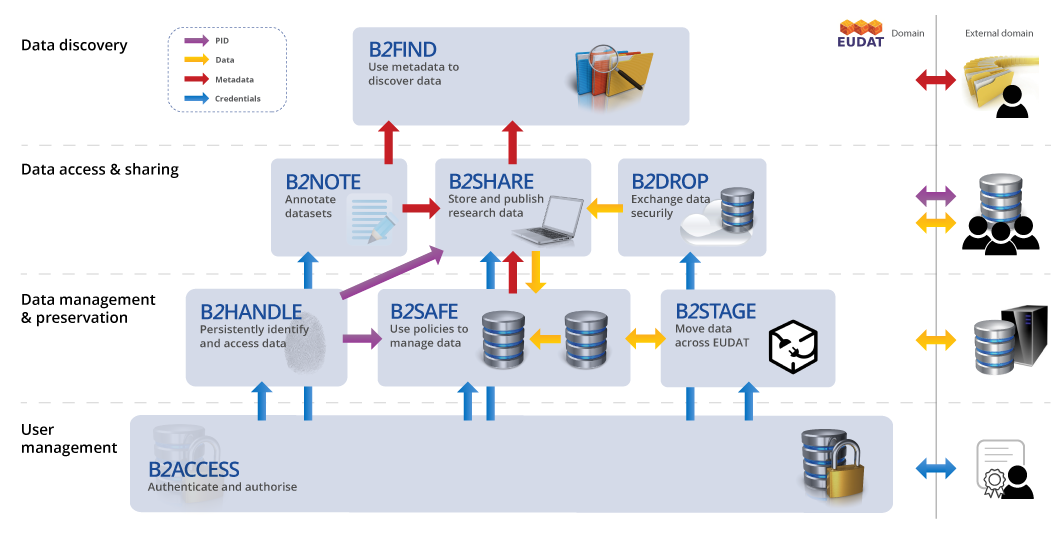
\includegraphics[width=1\textwidth]{img/state_of_the_art/eudat_services.png}
    \caption{\textit{\gls{eudat}} services (https://eudat.eu/services/userdoc/eudat-primer)}
    \label{fig:eudat_services}
\end{figure}
  
\subsubsection{Interaction with \textit{EUDAT} CDI}
  
 The users of the EUDAT common services appear in two layers: researchers as end-users and experts from the scientific communities/organisations \citep{damien}. 
 
 There are two ways in which scientific communities/organisations can integrate with \textit{\gls{eudat}}:

\begin{itemize}
    \item Join: community becomes a data centre or computing centre part of the \textit{\gls{eudat}} network, which is more demanding to develop, but allows close use with all core services. This requires a minimal installation and configuration of the \textit{\gls{eudat}} CDI, and the provision of some resources, such as computing and storage, by the community;
    \item Use: an existing \textit{\gls{eudat}} data centre or computing centre ingests the community data and ensures its storage and also its replication, if desired. Unlike the former, due to the looser interaction, users will have little or no control over the development of core features and their configurations. {\textit{\gls{eudat}}} exposes several UIs (to aggregate them, a {Common Services Layer Interface (CSLI)} is currently under development) and \gls{api}s for using its services.
\end{itemize}

End-users can also use the system in a similar way to community use, however, data replication is not possible for them.
  
\begin{figure}[!htb]
   \begin{minipage}{0.48\textwidth}
     \centering
     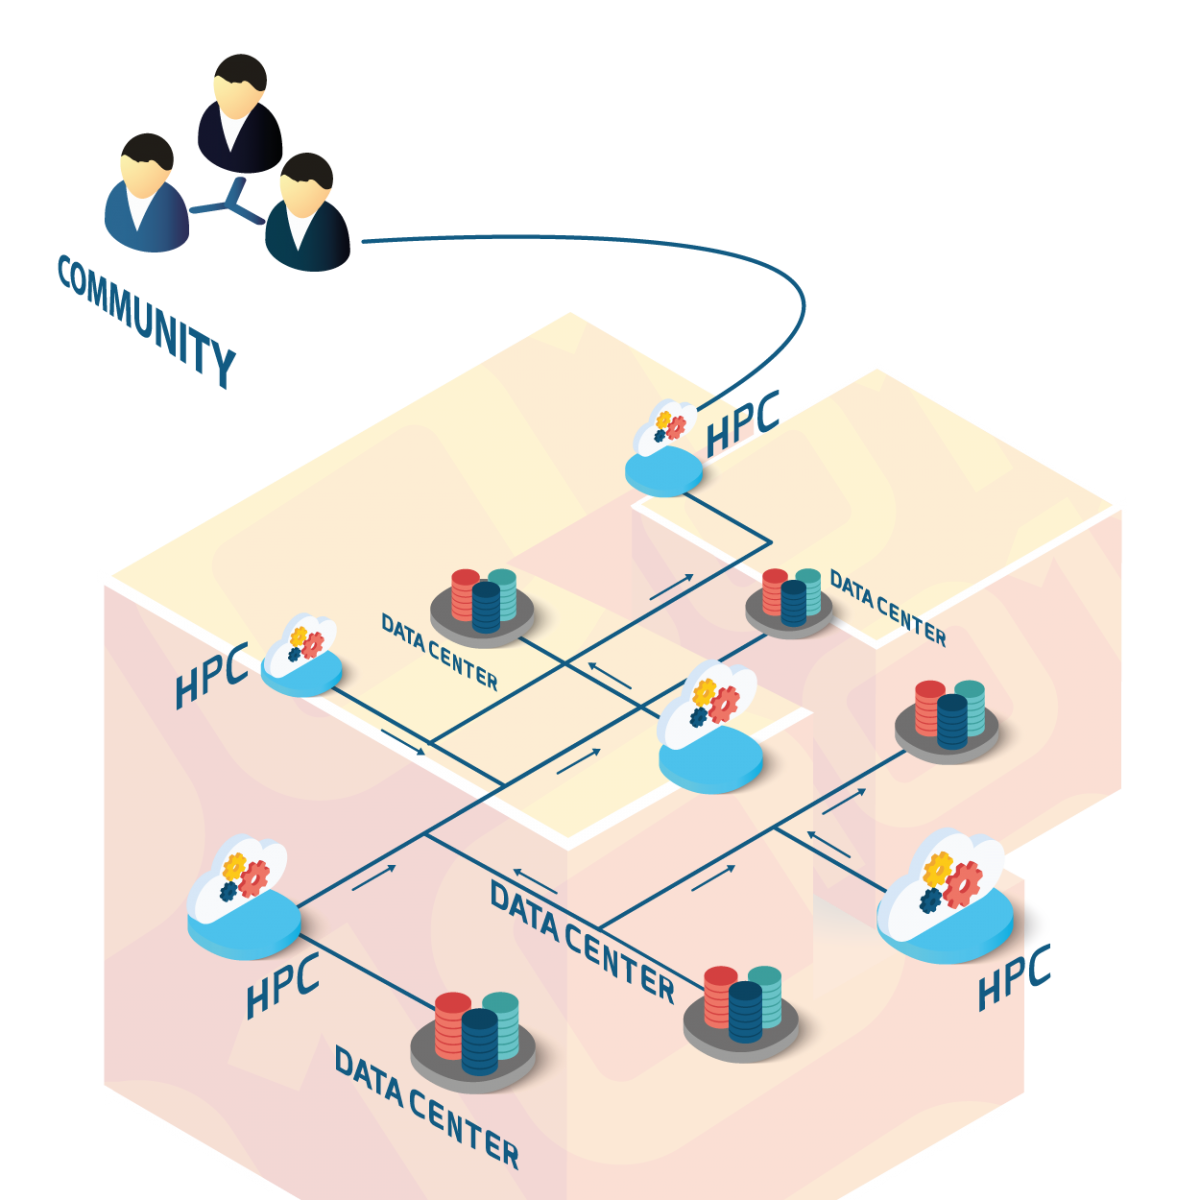
\includegraphics[width=0.85\textwidth]{img/state_of_the_art/use_eudat.png}
     \caption{Using the \textit{\gls{eudat}} services (https://www.eudat.eu/eudat-cdi/using)}\label{Fig:Data1}
   \end{minipage}\hfill
   \begin{minipage}{0.48\textwidth}
     \centering
     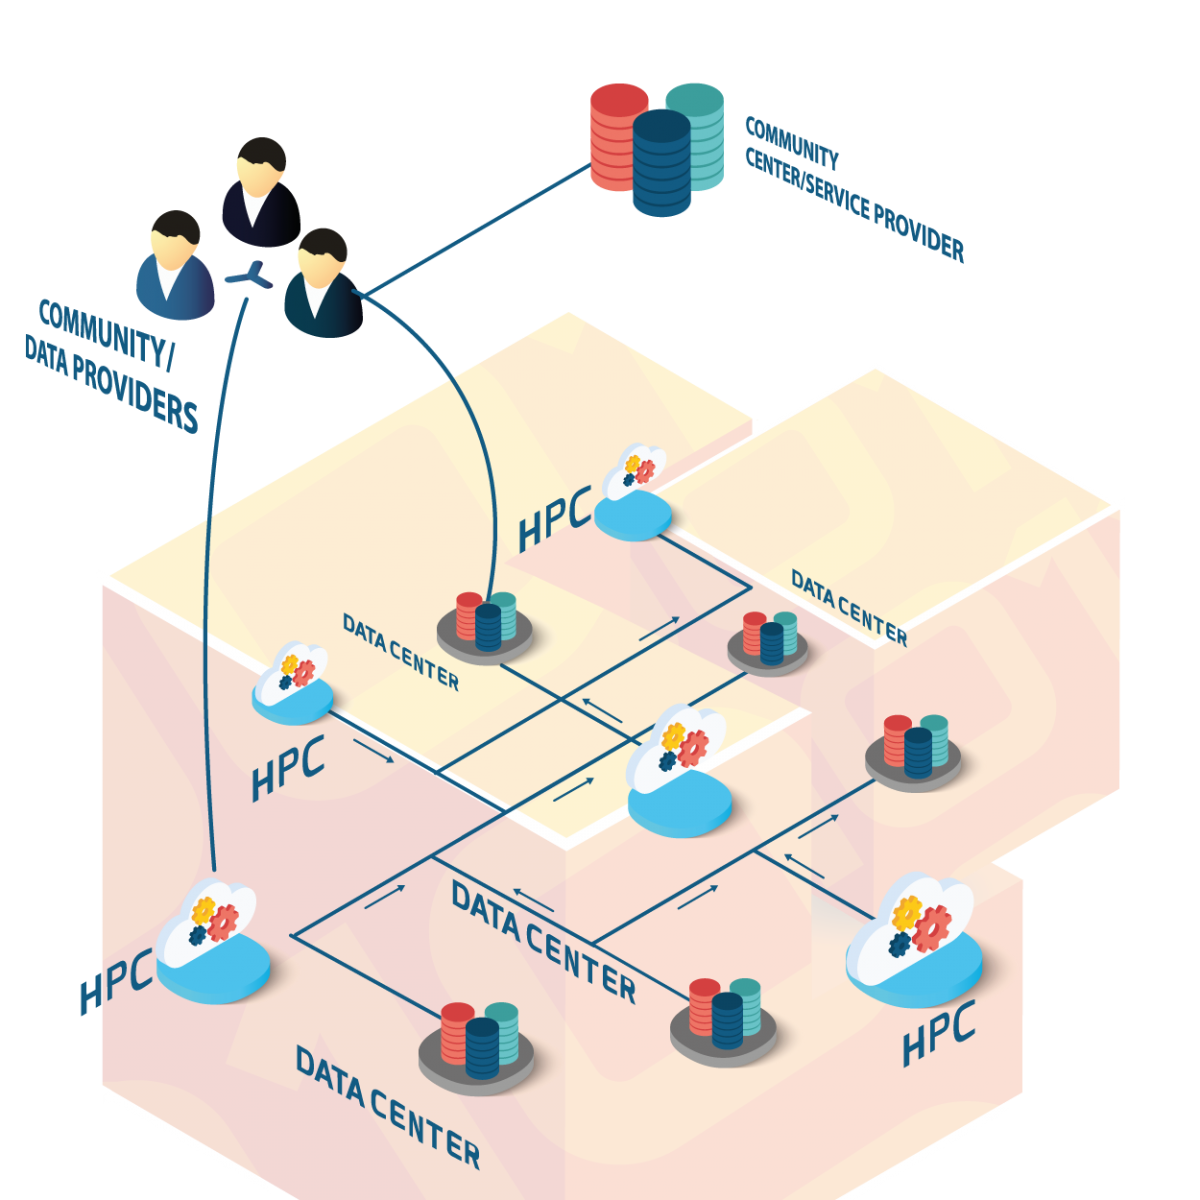
\includegraphics[width=0.85\textwidth]{img/state_of_the_art/join_eudat.png}
     \caption{Joining the \textit{\gls{eudat}} services (https://eudat.eu/eudat-cdi/joining)}\label{Fig:Data2}
   \end{minipage}
\end{figure}
  
In both cases, the community can access \textit{\gls{eudat}'s} primary services, which will be analysed in the next subsection. The following image clearly illustrates the distinction between the two forms of interaction.
  
\begin{figure}[!h]
    \centering
    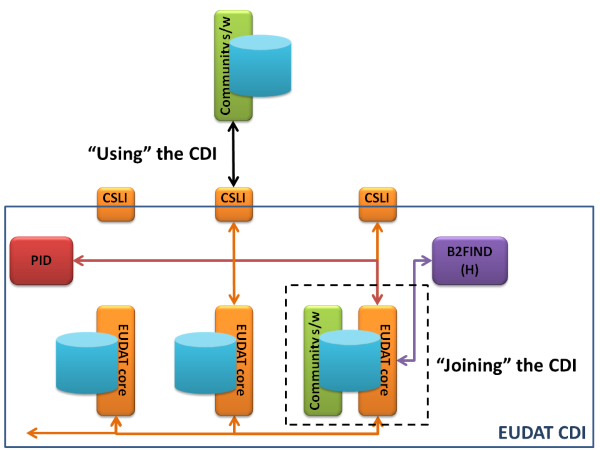
\includegraphics[width=0.6\textwidth]{img/state_of_the_art/use_or_join.png}
    \caption{Interaction with the \textit{\gls{eudat}} CDI (https://eudat.eu/services/userdoc/eudat-primer)}
\end{figure}
  
\newpage
  
\subsubsection{\textit{B2ACCESS}}
  
\label{tab:b2access}  
  
\textit{B2ACCESS} is a federated cross-infrastructure framework for user authentication and authorisation that controls their access to other services and resources.
  
Users can authenticate in several ways: 
  
\begin{itemize}
    \item User's home organisation identity provider;
    \item Social account, like \textit{Google} or \textit{Facebook};
    \item \textit{B2ACCESS} id.
\end{itemize}
  
The \textit{B2ACCESS} process is based on two  aspects - attributes and groups. Attributes are key-value pairs that describe basic user information, such as their name, and keep information for authorisation purposes, such as membership to communities. Groups are used to manipulate and control user's access to other services, with each service having its own set of groups.
  
\subsubsection{\textit{B2DROP}}
  
\textit{B2DROP} is a trustworthy service used by investigators to exchange data and thus keep data synchronised and up-to-date with each other, being based on \textit{NextCloud}.
\textit{B2DROP's} main intention is to be used for volatile data that can be easily change and still subjective for the research and to manage this provides the version of the inserted files but does not maintain persistent identifiers for them. It can be used via a user-friendly web UI or implemented as a drive on the desktop machine via WebDav.
    
\subsubsection{\textit{B2FIND}}
\label{tab:b2find}

Metadata is a key part of data management, as they describe the dataset. Systematically structured and searchable metadata enables efficient discovery of scientific data, and this is how \textit{B2FIND} service works, using a comprehensive joint metadata catalog and a search portal respectively, aided by \textit{\gls{ckan}} functionality and \gls{api}.
  
This service can be used through the discovery portal via the web, an \gls{api}, or an intuitive command-line tool, and encompasses advanced functions like presenting datasets through tables or filtering by location using geospatial features. To search by metadata there are three options, which can even be used together:
  
\begin{itemize}
  \item Free text search, without any restriction;
  \item Faceted search, through specific fields or properties;
  \item By location or time.
\end{itemize}
  
\textit{B2FIND} aggregates diverse metadata information from heterogeneous sources within \textit{\gls{eudat}}. Regarding protocols for metadata, the standard is OAI-PMH, but other formats are also possible. 
  
The metadata schema is based on \textit{DataCite} schema but is compatible with others, such as DublinCore. Currently it includes 26 elements with different levels of obligation: mandatory if applicable; recommended; optional. Some of these elements incorporate important particularities related to the content, such as the use of persistent identifiers of resources (the DOI being specifically intended to make citation available), or information about its licensing and consequent permission status for use by other researchers. 
  
The use of a metadata schema and collection protocols such as these add a validation component in the process of improving metadata quality, a process in which \textit{B2FIND} is embedded.
  
\subsubsection{\textit{B2HANDLE}}
  
\textit{B2HANDLE} is a distributed service that handles the management of Persistent Identifiers (PIDs) based on the \textit{Handle} system, a trusted and scalable software infrastructure used by data curators focused on identifier registration services to create and control identifiers of their resources. The \textit{Handle} system for referencing PIDs uses a string as a prefix and a suffix separated by a "/". 
  
Communities that join \textit{\gls{eudat}} and want to provide this service can do so in two ways: either the data center itself runs \textit{Handle} or they pass their prefix to a \textit{\gls{eudat}} partner to manage the control. Thus, \textit{B2HANDLE} improves interoperability and makes operations of other services easier.
  
Other \textit{\gls{eudat}} services use this to ensure access to data from a long-term perspective, as well as its maintenance. Specifically, \textit{B2FIND} and \textit{B2STAGE} use \textit{B2HANDLE} to query objects and \textit{B2SHARE} and \textit{B2SAFE} to create and manage the PIDs of the data objects they store.
    
\subsubsection{\textit{B2HOST}}
  
Some members of \textit{\gls{eudat}} service providers -- Tieteen Tietotekniikan Keskus Oy (CSC) , Jülich Research Centre (JUELICH), Max Planck Gesellschaft (RZG) and SURFsara Bv (SURFsara) -- offer computing resources from their data centres through a service hosting framework called \textit{B2HOST}. These resources provide communities the ability to deploy and work their data-driven applications and services on machines close to the location of the data storage, since extra computing power may be required when the volume of data is too large to be transferred or there may be licensing restrictions that do not allow data to be copied to third parties. 
    
\subsubsection{\textit{B2NOTE}}
  
\textit{B2NOTE} is \textit{\gls{eudat}'s} latest service and offers creation and control of annotations on online resources, which can be comments and/or pointers that provide extra information about a resource.
Three types of annotations are possible: a semantic tag; a free-text keyword for when a specific semantic term is not found; a free-text comment. These are stored and can later be searched, and the results can be viewed via UI and refined before being exported or as JSON-LD (JSON for linked data).

At the moment this service is still being finalised and is not integrated into the other services.

\subsubsection{\textit{B2SAFE}}
  
\textit{B2SAFE} is \textit{\gls{eudat}}'s service that provides long-term data preservation through replication to multiple backup sites to ensure data redundancy.
  
This service is implemented as an \textit{iRODS (Rule-Oriented Data System)} -- data management software used in research worldwide module -- with \textit{Handle} REST \gls{api} or the EPIC \gls{api} (system with the same purpose as \textit{Handle}) that serves for the creation and management of PIDs and also uses the \textit{iRODS} middleware to replicate datasets from a datacenter as a source. Communities can ask another \textit{\gls{eudat}} site to host this service and responsibility. 
  
Lastly, each data object, original or replica, is assigned with a PID, which even contains information connecting it to its parents if it is a replica, or to a list of direct children if it is the original.
    
\subsubsection{\textit{B2SHARE}}
  
\textit{B2SHARE} web-based service is a solution that ensures the long-term persistence of locally stored data and enables researchers to publish, store and share small or medium-sized datasets. This service uses other \textit{\gls{eudat}} services for data reliability and retention, while storage is managed by trusted nationally supported repositories.
   
Any user, registered or not, can search for data on the \textit{B2SHARE} homepage. However, it is also possible to deploy \textit{B2SHARE}, requiring a web server or cloud infrastructure as a well as a way to store the published data, and this same deployment can be done through \textit{Docker} containers. In addition, this service is the only one that is open-source.
  
This service has the particularity of being integrated with \textit{B2DROP}, which allows data to be added from it to \textit{B2SHARE}. Besides, the existing data in \textit{B2SHARE} can be searched through the search portal provided by \textit{B2FIND}, which harvests the metadata present in this service.
    
\subsubsection{\textit{B2STAGE}}
  
The \textit{B2STAGE} service offers data staging, in other words, the transfer of data between nodes for processing. There are two protocols for this: GridFTP for large datasets and HTTP for small to medium files.
  
Big Data computing manages a high volume of data and when there are several supercomputers involved is necessary to take data transfer even more seriously. The implementation of this service is currently limited to files managed by \textit{B2SAFE}, handling the dynamic replication of data to the \gls{hpc}s. It also provides a \textit{B2STAGE} HTTP \gls{api} for dynamic access to data for integration into specific community applications.
  
\subsection{Evaluation}
  
The evaluation of the three systems analysed in the previous section is done based on the criteria also listed in the previous section, and is provided in Table \ref{tab:arch_comparison} to \ref{tab:usa_sec_comparison}. It should be noted that for the last table, the first field regarding popularity instead of being evaluated with a (\checkmark) or (\xmark)  is evaluated in order of popularity. 
  
\textit{\gls{ckan}} is already sucessful in several cases of government data platforms such as the US, corporate data platforms such as Lego, and is also used by the European Data Portal's, whose commitment to open research data and learning is paramount, with over 35 countries involved. \textit{\gls{eudat}}, meanwhile, has more than 25 member, all data centers and research organizations, such as CERN (European Organization for Nuclear Research). Finally, \textit{Magda} has as its only case of success its initial goal, which was to develop a federal government data portal for the government of Australia.
  
\begin{table}[h!]
    \begin{threeparttable}[b]
    \centering
    \caption{\label{tab:arch_comparison}Architecture comparison}
    \begin{tabular}{>{\centering\arraybackslash}p{1.75cm}>{\centering\arraybackslash}>{\centering\arraybackslash}p{3.5cm}>{\centering\arraybackslash}p{1.5cm}>{\centering\arraybackslash}p{2.5cm}>{\centering\arraybackslash}p{1.8cm}>{\centering\arraybackslash}p{3cm}}
        \hline
        \textbf{Platform} & \textbf{Installation and deployment} & \textbf{Open Source} & \textbf{Storage Replication} & \textbf{Storage Location} & \textbf{Customisation}   \\ 
        \hline
        \textit{\gls{ckan}}              & Installation package or service &       \checkmark                 & \xmark                           & Local or remote\tnote{1}          & \checkmark                            \\
        \textit{Magda}             &  From source or service                     & \checkmark                             &  \xmark                         &  Local or remote                       &  \checkmark             \\
        \textit{\gls{eudat}}             &  Service                     & \xmark\tnote{2}                             &  \checkmark                         & Remote                    & \xmark    \\
        \hline
    \end{tabular}
    \begin{tablenotes}
       \item [1] Remote only available through extensions
       \item [2] Only one service supports this feature
     \end{tablenotes}
    \end{threeparttable}
\end{table}
 
  
\begin{table}[h!]
    \begin{threeparttable}[b]
    \centering
    \caption{\label{tab:int_metadata_comparison} Interoperability \& metadata comparison}
    \begin{tabular}{>{\centering\arraybackslash}p{1.6cm}>{\centering\arraybackslash}p{1cm}>{\centering\arraybackslash}p{2.25cm}>{\centering\arraybackslash}p{1.75cm}>{\centering\arraybackslash}p{2cm}>{\centering\arraybackslash}p{2cm}>{\centering\arraybackslash}p{1.25cm}>{\centering\arraybackslash}p{1.75cm}}
        \hline
        \textbf{Platform } & \textbf{\gls{api}s} & \textbf{Harvesting protocols} & \textbf{Standard schemas}  & \textbf{Validation} & \textbf{Federation} & \textbf{DOI} & \textbf{Licensing}  \\ 
        \hline
        \textit{\gls{ckan}}               & \checkmark           & \checkmark\tnote{1}  &  \checkmark\tnote{1}                       & \xmark                      & \checkmark\tnote{1}         & \checkmark\tnote{1} & \checkmark                       \\
        \textit{Magda}              &  \checkmark              & \xmark               & \xmark\tnote{2}               &  \xmark & \checkmark  &  \xmark  & \checkmark                                      \\
        \textit{\gls{eudat}}              &  \checkmark             & \checkmark             &  \checkmark               & \checkmark               & \checkmark &  \checkmark     & \checkmark                                \\
        \hline
    \end{tabular}
    \begin{tablenotes}
       \item [1] Only available through extensions
       \item [2] Only partially
     \end{tablenotes}
    \end{threeparttable}
\end{table}

\newpage


\begin{table}[h!]
    \centering
    \caption{\label{tab:usa_sec_comparison}Usability \& security comparison}
    \begin{tabular}{>{\centering\arraybackslash}p{1.75cm}>{\centering\arraybackslash}p{2cm}>{\centering\arraybackslash}p{2cm}>{\centering\arraybackslash}p{2cm}>{\centering\arraybackslash}p{4cm}>{\centering\arraybackslash}p{2cm}}
        \hline
        \textbf{Platform}  & \textbf{Popularity}  & \textbf{Advanced search} & \textbf{Geospatial tools} & \textbf{Authorised authentication} & \textbf{Curation workflow}   \\ 
        \hline
        \textit{\gls{ckan}}               & 1º                              & \checkmark                  & \checkmark                     & \checkmark  & \xmark                   \\
        \textit{Magda}              & 3º                      &  \checkmark                   &   \checkmark                  &         \xmark      & \xmark                                \\
        \textit{\gls{eudat}}              & 2º                     &   \checkmark                  & \checkmark                    &   \checkmark & \checkmark                      \\
        \hline
    \end{tabular}
\end{table}
  
After the analysis and evaluation, \textit{\gls{ckan}} is the one that stands out the most. Although it has more cases of proven success in the use made by government institutions for processing their data, the fact that it is an open-source system, has a wide range of features, powerful \gls{api}s, and the possibility of customisation and extensions of functionalities make it possible to use it as a \gls{sdms} \citep{1}. In addition, it gives the option (even incentive) to organisations to have full control over the storage of their data, which can be a key decision for many scientific institutions.

An interesting fact is also the use of \textit{\gls{ckan}} by the other two systems addressed, \textit{\gls{eudat}} in the use of the search portal and \textit{Magda} in metadata aggregation, which demonstrates its value as a solution for data management.
  
There would have been other criteria that could have been taken into account, but this dissertation has focused on those we considered to be the most important in the current choice of a system that is as efficient for large institutions as for smaller ones, whose community support in the development of the platform is somewhat advantageous. 

Apart from the evaluated systems, i.e. \textit{\gls{ckan}}, \textit{Magda} and \textit{\gls{eudat}}, we enunciate other solutions that would be interesting to analyse, such as:
  
\begin{itemize}
    \item \textit{DSpace}, which focuses on creating open source repositories for scholarly and published digital content and shows a few similarities to what \textit{\gls{ckan}} offers. This software package was developed by MIT and HP Labs and has notorious examples of its use such as Apollo (Cambridge University repository) or the Open Knowledge Repository (World Bank repository);
    \item \textit{Invenio}, an open source repository software offering tools for managing digital content in institutional repositories and research data management systems (RDMSs). It was initially developed by CERN, but is also used by other institutions such as the SLAC National Accelerator Laboratory, a U.S. Department of Energy laboratory operated by Stanford University;
    \item \textit{Dataverse}, an open source web application similar to \textit{\gls{ckan}}, but with a greater focus on research data. This project was developed by an institute at Harvard University and of particular note is its use as national solutions for university repositories, proven, for example, in the Netherlands and currently being developed in Norway.
\end{itemize}

Finally, before we proceed to the development of a \textit{\gls{ckan}} based system and its consequent qualitative and quantitative evaluation, we will qualitatively evaluate a \textit{\gls{eudat}} system adapted to our case study. As we have seen in this chapter, the potential of \textit{\gls{eudat}} in the future, if made available for development, could be even more powerful than the \textit{\gls{ckan}} system, so it is in our interest to understand how we could set it up.

\subsubsection{EUDAT}

We now address how our system, which will be developed through \textit{\gls{ckan}}, could have been developed in \textit{\gls{eudat}}. It would also be interesting for us to make a quantitative evaluation, but after contacting the \textit{\gls{eudat}} team, they were inflexible in providing unlimited access to their services for local development purposes, since their integration policy is somewhat rigid. Despite this, they have some workloads for some of their services to be developed locally, but mostly without any support or with the need to get in touch with communities of other software.

Through the experience we have gained through the use of \textit{\gls{eudat}} services in production mode, and through some local reproductions of some of its services, we have been able to understand how we can take advantage of the system considering our case study. We therefore examined which services would be interesting to implement:

\begin{enumerate}
    \item \textit{B2ACCESS}: in order to take advantage of most \textit{\gls{eudat}} services, it is necessary to register on the platform responsible for simple and secure authentication and authorisation. There are several possibilities for authentication, however, we can take advantage of \gls{inesctec}'s existence as an organisation already inserted in the system and authenticate ourselves by providing the identity of the user's organisation of origin. Therefore, it is already possible to access the remaining services without any restriction;
    \item \textit{B2DROP}: after accessing \textit{\gls{eudat}}, the first service to use would be \textit{B2DROP}, which is used to store and exchange data between colleagues in the research team. In this case, the data to be stored in this service would be \gls{gnss} and \gls{nmea}, as these formats do not allow their usability and would need to be processed. This platform allows the insertion of files with a maximum of 2 GB and each user has a maximum quota of 20 GB, which we believe would fit the amount of information resulting from the \gls{sail} Project;
    \item \textit{B2SHARE}: Once we have considered the \textit{B2DROP}, it makes sense to understand where we could store and publish the already processed data, this is where \textit{B2SHARE} comes in, which serves that purpose. In addition, it guarantees the long-term preservation of that same data (through a PID associated to the dataset), which is ideal for those we already consider as final such as the CSV files of the measurements of atmospheric conditions. Thus, while \textit{B2DROP} does not allow metadata, \textit{B2SHARE} already does, and so we could enjoy the use of time and location as some of the fields. When it comes to values, \textit{B2SHARE} allows to upload files up to 10GB and records up to 20GB;
    \item \textit{B2HANDLE}: the acquisition and management of the PIDs made by this service can be entrusted to the \textit{B2HANDLE} team, it is only necessary to acquire a production prefix, which is requested to the team through a form;
    \item \textit{B2FIND}: Although \textit{B2SHARE} shares data and we can search through its platform, this is limited, since its purpose is not that. However, this component is important in the research project of \gls{sail} and, then, the use of \textit{B2FIND} arises, which harvests metadata from different sources, including \textit{B2SHARE}, and includes a data portal (based on \textit{\gls{ckan}}) that allows searching them. To publish the metadata in \textit{B2FIND} it is not enough to have them in \textit{B2SHARE}, we must take into account the protocol we offer to provide the metadata, which is preferably the OAI-PMH protocol, and their schema. Regarding the first point, the OAI-PMH protocol has already been taken into account when preparing the \gls{sail} data management plan and, regarding the second point, one of the schemas considered in that same plan is Dublin Core, which is one of the formats recognised by \textit{\gls{eudat}}. As such, no change would be necessary and it would be sufficient to have the metadata present in \textit{B2SHARE}. 
\end{enumerate}

After evaluating these services, we summarize the reasons why we would not consider the rest in the integration of a system adapted to \textit{\gls{eudat}}:

\begin{enumerate}
    \item \textit{B2NOTE}: the possibility to have annotations to resources is something interesting and that we could contemplate in the system, but it is not yet integrated in \textit{\gls{eudat}} services and is therefore unavailable;
    \item \textit{B2SAFE}: this service emerges as a solution for communities without archiving facilities or without considerable computing resources, which basically need to replicate their data in different data stores. This is not the case in our situation, because an infrastructure like \gls{macc} would have the resources to take control of the system;
    \item \textit{B2STAGE}: required to transfer data in an \gls{hpc} environment, between different data stores, which would be useful when using the \textit{B2SAFE} service.
\end{enumerate}
  

        
\chapter{Research data repository}

    \label{ref:chapter_3}

This chapter covers the solution developed for the problem presented in this thesis, from how it is implemented, addressing the particularities of the case study and its data, to the obstacles encountered and the improvements made to the \textit{\gls{ckan}} base system.

After the definition of \textit{\gls{ckan}} as the system to be adopted, the investigation of the functionalities to be considered for the \gls{sail} Project had a new contribution from its team, who informed us about the key elements to be considered in the elaboration of the system, taking into account the nature and usability of the data:
  
  \begin{enumerate}
      \item Understand how best to organize the data;
      \item View data geographically;
      \item Filter the data geographically;
      \item Restrict content according to user type;
      \item Seek to integrate \textit{\gls{eudat}}, more specifically the \textit{B2FIND} service.
  \end{enumerate}


    \section{Deployment}
    
        First of all, we describe the requirements for deploying the software on a new machine, as well as a step-by-step approach to try it out.

\newpage

For the installation of the system it is necessary to meet certain prerequisites, which are listed below:

\begin{itemize}
    \item Unrestricted access to external domains, such as \textit{GitHub} or \textit{DockerHub};
    \item Have docker, docker-compose and git installed;
\end{itemize}

Once the prerequisites listed above are met, we need to download the software as well as some custom images to run certain docker containers. For this, we need to run the following commands:

\begin{itemize}
    \item Clone \textit{\gls{ckan}} into a directory of choice:
        \begin{verbatim}
cd /path/to/directory
git clone https://github.com/priest110/ckan.git
        \end{verbatim}
    \item Pull the required docker images from the \textit{DockerHub}:
        \begin{verbatim}
docker pull priest110/docker_db:1.0.0
docker pull priest110/docker_ckan:1.0.0
        \end{verbatim}    
\end{itemize}

Reaching this point, we have a working system, however, the \textit{Docker} installation has a problem regarding the recognition of localhost as a valid address (where the main service \textit{\gls{ckan}} is running) for other services, in this case for the \textit{Datapusher}, which makes it impossible to run well. As such, some changes need to be made to the hosts file:

\begin{enumerate}
    \item First, find the IP 0f the docker0 bridge:
    \begin{verbatim}
ip addr show | grep docker0
    \end{verbatim}
    \item An example of the possible output:
    \begin{verbatim}
10: docker0: <NO-CARRIER,BROADCAST,MULTICAST,UP> mtu 1500 qdisc noqueue state 
DOWN group default 
    inet 172.17.0.1/16 brd 172.17.255.255 scope global docker0:
    \end{verbatim}
    \item Next, we can then edit /etc/hosts/ file:
    \begin{verbatim}
172.17.0.1 dockerhost
    \end{verbatim}
    \item Restart the \textit{Docker} daemon:
    \begin{verbatim}
sudo service docker restart
    \end{verbatim}
    \item Run:
    \begin{verbatim}
docker-compose -f docker-compose.yml -f docker-compose.override.yml up -d
    \end{verbatim}
\end{enumerate}

After this, we have all the services working well, just navigate to http://dockerhost:5000 and explore.



    \section{Data}
    
        The organisation of the data was an important aspect to consider when developing the solution, taking into account the structure and nomenclature defined in Subsection \ref{tab:sail_project}.

To take advantage of the usability, before inserting the datasets we tried to match the features of \textit{\gls{ckan}} to what we wanted from the data. As such, we first took the preprocessed data sample and converted it to a CSV format, since \textit{\gls{ckan}} tools allow geospatial availability and interaction with it from structured data, and provide other formats that are also interesting for us to analyse the data, such as table and graph. Thus, we are able to test the usability of the data with geospatial fields, with the help of extensions, which we will talk about later. With regard to the raw \gls{gnss} and \gls{nmea} data, it would also be possible for us to convert it to CSV and make it viewable, however, it is purely data associated with location and time, whereas the structure data associates location with other data relating to atmospheric conditions, so we have chosen to keep the \gls{gnss} and \gls{nmea} data in the original format.

We have organised the information into 3 different types of datasets, whose titles are as follows:

\begin{itemize}
    \item Structured atmospheric measurements;
    \item Raw \gls{gnss} measurements (YYYY/MM/DD);
    \item Raw \gls{nmea} measurements (YYYY/MM/DD).
\end{itemize}

For each type of dataset, we have several datasets encompassing daily information regarding \gls{gnss} and \gls{nmea} measurements, and one dataset for the structured data since our preprocessed sample has only 6 files, each one on a different atmospheric condition. However, it would make sense to adopt the same behaviour for the structured data with a sample of the same size as the other measurements, and consider a different daily dataset for each atmospheric condition.

At this point, we can already see that we will have dozens and dozens of datasets, since they are daily datasets. As such, we chose to insert the date in the title so that not all datasets have the same name and it also allows us to find any dataset through a search in \textit{\gls{ckan}'s} search engine, for example, if we search for "title:23", all datasets that have 23 in the title will appear, including the datasets that have the day 23. However, if we choose to search for "title:10" will already appear datasets with month equal to 10 and/or day equal to 10, therefore, we chose to add 3 key-value pairs to the metadata, being the keys "year", "month" and "day", so if we search for "day:10 month:01" will effectively only appear the datasets associated with day 10 of month 01.

Finally, besides the datasets and respective files, we also included in the system 2 organisations -- \gls{inesctec} and High-Assurance Software Laboratory (HASLab), which is one of \gls{inesctec}'s integrated R\&D centres -- and 1 group -- \gls{sail} Project. While it is necessary in \textit{\gls{ckan}} to have an organisation that owns and manages the information, in this case study, \gls{inesctec}, there is no need for groups, however, they can be used in order to catalogue a team, theme or project, in this case \gls{sail} Project.
        
    \section{User Interface (UI)}
    
        We have chosen to make some changes in the User Interface available in the front-end in order to take advantage of the features provided by \textit{\gls{ckan}}. In what concerns the pages alluding to datasets and resources, as well as those of groups and organisations, we consider that the information is already provided in an intuitive way and, in our opinion, does not need any changes. Nevertheless, we consider that the homepage could suffer some changes, and, as such, we opted to work on it and obtained the result shown in the figure \ref{tab:homepage}.

\begin{figure}[!h]
    \centering
    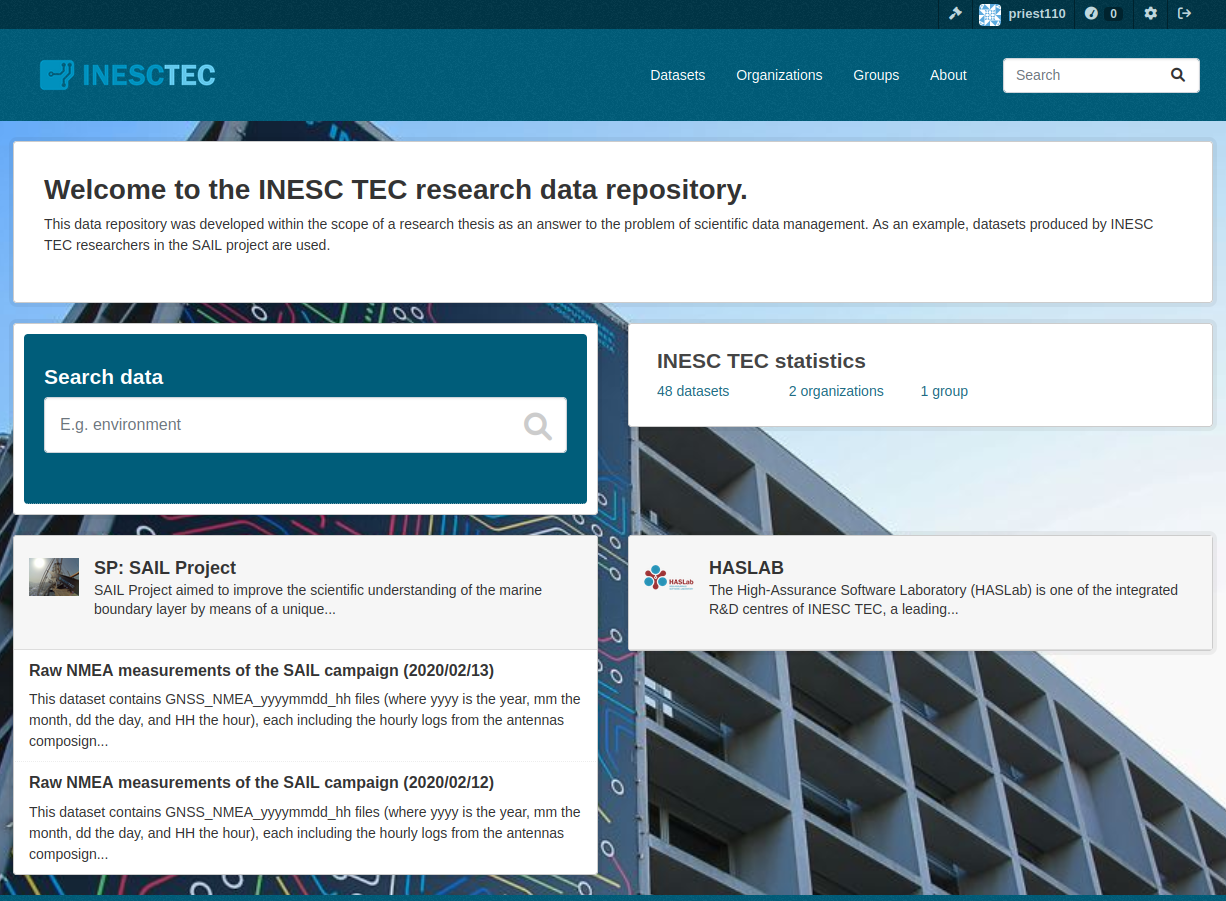
\includegraphics[width=1\textwidth]{img/solution/UI.png}
    \caption{\label{tab:homepage} Homepage}
\end{figure}

Thus, we have improved the initial aesthetics of the main page (which ends up being the first thing that users will see in the system) and we have customised it to fit in with the institution that uses its services. Furthermore, as the primary reason for the change, we have been able to transmit more useful information, as previously only the welcome statement, the search engine, and the statistics were considered, and now it is also possible to access two additional components:

\begin{itemize}
    \item Latest group in the system, in this case associated with \gls{sail} Project, and its two latest resources;
    \item The most recent organization in the system, which is HASLab, and which in turn does not yet have any associated resources.
\end{itemize}
        
    \section{Extensions}
    
          One of the great advantages of \textit{\gls{ckan}} is effectively its customisation and the existence of numerous solutions developed for use as extensions to its base system. As such, we examined which extensions could be interesting to explore in our case study, as well as the outcomes and consequences of their implementations.
  
  \subsubsection{ckanext-spatial}
  
  This extension, along with ckanext-geoview, are undoubtedly the ones that had the greatest impact meeting the requirements of the \gls{sail} Project, because they allowed answers to two of the five questions posed at the start of the chapter. More specifically, the geospatial capabilities that this extension added to the system include:
  
  \begin{itemize}
      \item A new field ("spatial") in the dataset metadata schema, which allows this same field to be available through a map on the front-end of the dataset's respective page, and also geospatial queries, such as filtering by geographic area;
      \item Harvesters to import geospatial metadata from other sources into \textit{\gls{ckan}}.
  \end{itemize}
  
  As for the same dataset we have several files with different latitudes and longitudes, we have chosen to collect the information regarding the maximum and minimum values of each measure. Thus, we obtain an area relative to the investigation of each day, this area being the value of the "spatial" key, which after adding to the metadata is ready to be viewed.

  \subsubsection{ckanext-geoview}
  
  This extension contains view plugins to display geospatial files and services in \textit{\gls{ckan}}. Thus, it made it possible for all resources with structured data with latitude and longitude fields to be viewed through a geographical map, and also provided filtering capabilities, for example, in the number of entries to be viewed in a given file, and interaction, for example, in the ability through the map to access a particular climatic condition associated with a geographical point.
  
  \subsubsection{ckanext-harvest}
  
  Although this is not something essential to consider for a project like the one we are addressing, we believe that this extension will add quality to any system that manages data, as it allows us to generate datasets from other sources.

  For instance, considering that some research team outside \gls{inesctec} would like to access some of the data provided by the \gls{sail} project in order to explore it further or in a different way, new information could emerge that \gls{inesctec} would consider interesting to make available on its platform. For that, it would be enough to use a harvester to fetch the remote dataset from where the new data would be into our system.
  
  After adding the harvester, we can define if we want to run it weekly, daily, annually, and each time we do it the following happens:
  
  \begin{itemize}
      \item New datasets will be added locally, if any;
      \item Updates that are done on the remote datasets, will also be done locally;
      \item Datasets that no longer exist remotely will be deleted locally.
  \end{itemize}
  
  \subsubsection{ckanext-doi}
  
  We have added this extension to assign a DOI when a dataset is created and made public. This requires an account at \textit{DataCite}, since it is the service that handles the assignment. Note that the DOI is in the format:
  
  \begin{verbatim}
  https://doi.org/[prefix]/[8 random alphanumeric characters]
  \end{verbatim}
  
  Again, for this project this extension would not have the best of uses, as it would assign different DOI's to each dataset, when they are all part of the same investigation. As such, it would be useful to have a DOI, but in this case this would be the same for all datasets and would have to be assigned outside the system (whereby we could use the existing https://doi.org/10.5281/zenodo.5797919 referring to the \gls{sail} Project). However, this extension would be extremely useful in most cases.
  
  \subsubsection{ckanext-dataspatial}
  
  This extension is no longer maintained and unfortunately no longer works for the version of \textit{\gls{ckan}} we are using, however, like others mentioned, while interesting, it is not core. 

  It would provide geospatial awareness of \textit{DataStore} data, which includes geospatial searches within datasets and the spatial extension of \textit{DataStore} searches. However, the first of the two capabilities can be achieved through ckanext-geoview.
  
  \subsubsection{ckanext-hierarchy}
  
 Often there are relationships between organizations, like the one we contemplate in our system, for example, since HASLab is an organization that belongs to \gls{inesctec}. However, in the default \textit{\gls{ckan}} system there is no way to make explicit the relationship between two or more organizations, so we chose to use this extension, which allows us to:
  
  \begin{itemize}
      \item Create relationships between organisations;
      \item Hierarchize the relationships;
      \item For each organisation, on its datasets page, in addition to having available the ones it owns, we can choose to also provide the datasets of the organisations it owns.
  \end{itemize}
  
  \subsubsection{ckanext-restricted}
  
  Through this extension we were able to answer one more of the points listed at the beginning of the chapter, since it provides the possibility of restricting access to resources in a dataset, while still being able to view the metadata but not the data itself. However, this extension is currently out of date, which does not allow proper use.
  
  The access levels that we can assign to the resources in a dataset are as follows:
  
  \begin{itemize}
      \item Public;
      \item Registered users;
      \item Members of an organization;
      \item Members of the organization that owns the dataset.
  \end{itemize}
  
  \subsubsection{ckanext-oaipmh}
  
  Aside from the sources provided by the ckanext-harvest extension, this extends the \textit{\gls{ckan}} harvester to parse OAI-PMH metadata sources as well as import datasets. It supports metadata schemas such as oai\_dc (Dublin Core), used in the \gls{sail} project.
  
  This extension is outdated and, since it is not supported by the \textit{\gls{ckan}} team (it was developed by the community), it should not be updated again for the new \textit{\gls{ckan}} version. As such, there are some bugs that do not allow its proper use.
  
  \subsubsection{ckanext-b2find}
  
   The \textit{B2FIND} service, already discussed in Section \ref{tab:b2find} provides a user-friendly data discovery portal to search for research information stored in various repositories.
 
   This extension allows the use of the \textit{B2FIND} service on \textit{\gls{ckan}}, which in essence ends up allowing a different approach to metadata aggregation, since the search portal is based on \textit{\gls{ckan}}. 
   
   Like others already mentioned, this extension is outdated, but it is currently in transition progress, and we estimate that in a few months it will be possible to enjoy its functionalities. 
  
  \subsubsection{ckanext-ord-hierarchy}
  
  Finally, this last extension is similar to ckanext-hierarchy, however, it is used to create and provide relationships between datasets through a hierarchy. Looking at the way we have structured the datasets, we believe that there are no ownership relations between them, however, it is another extension that brings quality to the system and could easily be considered for other cases.

  \newpage
    
    \section{Discussion}
    
        There were several obstacles encountered during the development of the solution, and some have already been addressed throughout the chapter, but we opted to dedicate this section to explore in more detail those in which we invested more time or which had more consequences on the final result.

The first challenge occurred in installing \textit{\gls{ckan}}, since, on the one hand, the latest stable version of it installed via \textit{Docker} uses \textit{Python} 2, which is no longer supported, while, on the other hand, the master version is in transition to \textit{\textit{\gls{ckan}}} 2.10. We ended up choosing the second option because, after contacting the \textit{\gls{ckan}} team, they informed us that they believed the master version was stable enough, and, in addition, had the advantage of working with \textit{Python} 3.
  
As far as extensions are concerned, there were several that did not work, since they are outdated (ckanext-restricted, ckanext-dataspatial, ckankext-ord-hierarchy, ckanext-oaipmh), or have limited functionality (ckanext-b2find), and therefore could not be used. However, although they added quality to the software they were not central to what we wanted to develop, and we believe that the most important extensions are present in the system.
 
Finally, the biggest obstacle was not being able to take advantage of the partnership with \gls{macc}, for reasons unrelated to the research. For this reason, it was not possible to recreate the best scenario regarding an \gls{hpc} environment. As such, we resorted to using machines from \gls{inesctec} to evaluate the performance of the developed system, which did not allow us to recreate an effective approximation to the real world, as would happen with the \gls{macc} resources.
        
\chapter{Performance Evaluation}

    \label{ref:chapter_4}

  In order to understand how the system behaves in a real-world context, especially to extrapolate its behavior on a large-scale system with thousands of requests per second, we need to understand how the system works in a much smaller, controlled world. To this end, we performed tests to obtain the server execution profile and, in this section, we will explain the test conditions, the methodology used, and the results we obtained from our adapted \textit{\gls{ckan}} system.
        
    \section{Test conditions and Methodology}
    
        To test the system, we used one of the machines from the \gls{inesctec}, specifically described in Table \ref{tab:machine}.

  
  \begin{table}[H]
    \centering
    \begin{tabular}{|l|l|}
      \hline
      \textbf{CPU   }        & Intel® Xeon® E5-2698 v4         \\ \hline
      \textbf{\#Sockets}          & 2                              \\ \hline
      \textbf{\#Cores per socket}          & 20                              \\ \hline  
      \textbf{\#Threads per core}          & 2                              \\ \hline
      \textbf{CPU Frequency}       & 2.2 GHz (base), 3.60 GHz (max.) \\ \hline
      \textbf{Memory}          & 32 GB DDR4-2400             \\ \hline
    \end{tabular}
    \caption{\label{tab:machine}Description of the machine used}
  \end{table}
  
  We used the \textit{Locust} \citep{loc} tool and the iostat command for testing. On the one hand, \textit{Locust} is a load testing tool developed in \textit{Python} that allows us to run tests in a distributed way across multiple machines and simulate thousands of users making requests concurrently. It produces two metrics: throughput, i.e. the number of requests the server can handle in a unit of time, and the response time, i.e. the time the server takes from the time it receives a request until it answers it (these two metrics seem to be the inverse of each other, but they are not, since throughput is very much limited by the number of requests we can launch per unit of time, while response time will be limited by the server's processing and resource management capacity). On the other hand, the iostat command is used for monitoring system input/output devices by observing the time they are active in relation to their respective average transfer rates, and allowed us to extract information regarding two other metrics: CPU and Disk utilisation.
   
  The tests were done using a variable number of clients, specifically from 0 to 1000, and the increment was divided into 3 stages:
  \begin{itemize}
      \item 0 to 100 concurrent users with a ramp up speed of 2 users/second;
      \item 100 to 500 concurrent users with a ramp up speed of 4 users/second;
      \item 500 to 1000 concurrent users with a ramp up speed of 6 users/second.
  \end{itemize}
  
  The interval from 0 to 1000 was chosen since from 1000 users on, and even before that, in some cases, there were already system faults (and not failures) due to the considerable weight of certain requests, which had the usual consequence of exceeding the timeout that we consider to be adequate in the response to a read request made to the server -- 5 seconds. Nevertheless, this interval proved to be more than enough to understand how the system responds, taking into account the hardware and the different types of requests used (shown in Table \ref{tab:type_requests}), where not all possible ones were contemplated, we neglected those that we considered to have no real relevance to reliably measure the performance of the system on a large scale. When it comes to the choice of using different stages, the goal was to understand the system's ability to adapt to different quantities and growths of users.
  
  \newpage
  
  \begin{table}[H]
    \centering
    \begin{tabular}{|>{\centering\arraybackslash}p{1.25cm}|>{\centering\arraybackslash}p{7cm}|>{\centering\arraybackslash}p{4cm}|>{\centering\arraybackslash}p{2.25cm}|}
      \hline
      \textbf{Type} & \textbf{URL (with prefix /api/3/action)} &  \textbf{Description} & \textbf{Probability}
      \\ \hline
      GET   & /current\_package\_list\_with\_resources
            & \begin{tabular}[c]{@{}l@{}}Return a list of the \\site’s datasets and \\their resources\end{tabular} 
            & 5       
            \\ \hline
      GET   & /package\_show?id
            & \begin{tabular}[c]{@{}l@{}}Return the metadata \\of a dataset and its \\resources\end{tabular}
            & 5   
            \\ \hline
      GET   & /resource\_show?id 
            & \begin{tabular}[c]{@{}l@{}}Return the metadata \\of a resource  \end{tabular} 
            & 4
            \\ \hline
      GET   & /group\_list 
            & \begin{tabular}[c]{@{}l@{}}Return a list of the\\ names of the site’s\\ groups\end{tabular} 
            & 3         
            \\ \hline
      GET   & /organization\_list
            & \begin{tabular}[c]{@{}l@{}}Return a list of the\\ names of the site’s \\organisations\end{tabular}  
            & 3         
            \\ \hline
      POST  & /package\_create
            & Creates a new dataset 
            &     
            \\ \cline{1-3}
      POST  & /package\_revise
            & \begin{tabular}[c]{@{}l@{}}Revise a dataset \\selectively\\ with match, filter and \\update parameters\end{tabular}
            & 1
            \\ \cline{1-3}
      POST  & /resource\_create\_default\_resource\_views 
            & \begin{tabular}[c]{@{}l@{}}Creates the default \\views (if necessary) on \\the provided resource\end{tabular} 
            &       
            \\ \cline{1-3}
      POST  & /datastore\_create 
            & \begin{tabular}[c]{@{}l@{}}Adds a new table\\ to the \textit{DataStore}\end{tabular} 
            &      
            \\ \hline
    \end{tabular}
    \caption{\label{tab:type_requests}Types of requests}
  \end{table}
  % \usepackage{multirow}

  
  All the core functionality of the site provided by \textit{\gls{ckan}} can be used through external code that invokes the \gls{api}, which will be extremely useful in testing. As such, the requests listed in the table above make use of the strong \gls{api} that \textit{\gls{ckan}} provides, which unlike requests made through the  web UI, do not need to load any views or templates. Also, for testing purposes, POST requests can only be recreated through the \gls{api}, so in order to get a fair comparison between requests, we chose to use only the \gls{api} to evaluate performance.

   
  Until we got to a realistic case, developing the tests required a cycle of optimizing/measuring the results in order to build a real test of an efficient server. As such, we divided the evaluation moments into three distinct ones:
  
  
  \begin{enumerate}
   \item Individual case, to understand how the system worked with just one individual type of request;
   \item Preliminary case, where we worked only with read-only requests, since in our view they are the ones that exist more frequently in the system and allowed us to get a sense of how it works while analysing other influencing factors based on the server and test tool settings:
   \begin{enumerate}
        \item waiting time between requests
        \item load distribution
        \item connection pool
   \end{enumerate}
   \item Realistic case with read and write requests, each request with a specific probability of occurring, since there are requests that are more frequent than others.
  \end{enumerate}
    
  \label{tab:request_factors}

  The instrumentation methodology, is as follows: we run a script with the \textit{Locust} that creates users and each one executes tasks, one at a time, until a voluntary stop is made, more specifically, about 10s after we get the 1000 users (each test took, on average, 4 minutes and 30 seconds). Each read request is included in a different task, while the four write requests are included in a single task, since for each insertion of new non empty dataset, we need one to create the dataset and another to add a certain resource, and besides different requests for each insertion, it is necessary to create default views for the resource, as well as add it to the \textit{DataStore} (the latter two allow the resources to be viewed and exploitable). It should be noted that each test was repeated several times in order to understand if the values presented were valid or suffered from some extraneous anomaly.
  
  \newpage
        
    \section{Individual case}
    
          Before we understand how the requests work together, it makes sense to understand their individual behavior, i.e., to consider the case where we make only a certain request, since certain decisions in later testing may be influenced by the behavior we observe in these first tests. For the POST requests, since we encompassed them all in one task, we consider all 4 as one type, and due to the heavy computation (4 different requests, as well as the random generation of the dataset and file to be uploaded to the platform), we chose to run only up to 100 users, which will serve to fully understand how they work.
  
  \subsection{Throughput}
  
  The first metric we evaluated was the throughput of requests that the server can answer, per second. This metric provides a notion of the system's behavior for a varied amount of clients, which will give us an idea of what would be the ideal number of simultaneous users corresponding to the highest number of answered requests per second.
  
  In Figures \ref{tab:throughput_datasets}, \ref{tab:throughput_groups_org} and  \ref{tab:throughput_write} we present the data collected in the tests with regard to throughput, and we chose to split the information between 3 different graphs (requests to read datasets and resources, requests to read organizations and groups, and write requests), since everything in the same graph would greatly reduce the perception of the results.
  
  \begin{figure}[H]
    \centering
    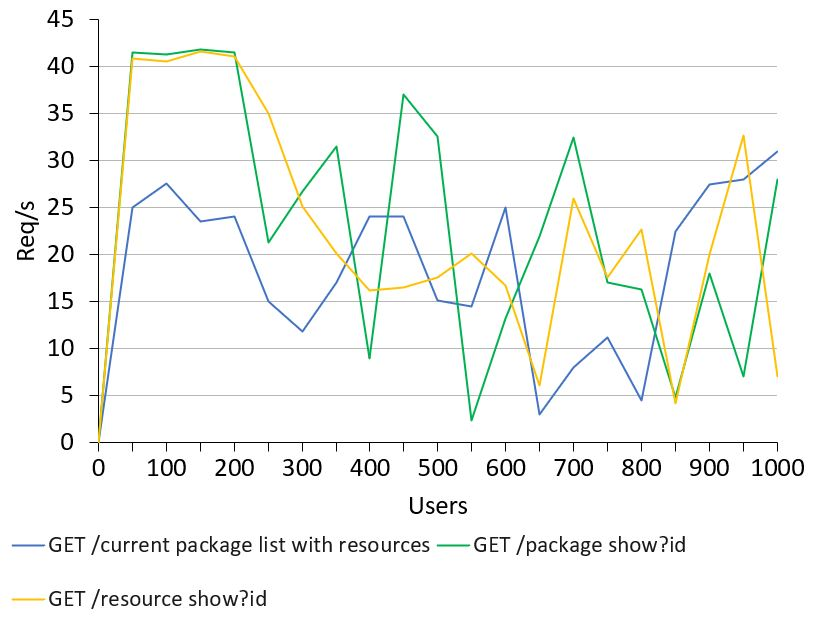
\includegraphics[width=.69\textwidth]{img/performance_evaluation/datasets_individuais.JPG}
    \caption{\label{tab:throughput_datasets}Throughput for dataset and resource requests}
  \end{figure}
  
  
  \begin{figure}[H]
    \centering
    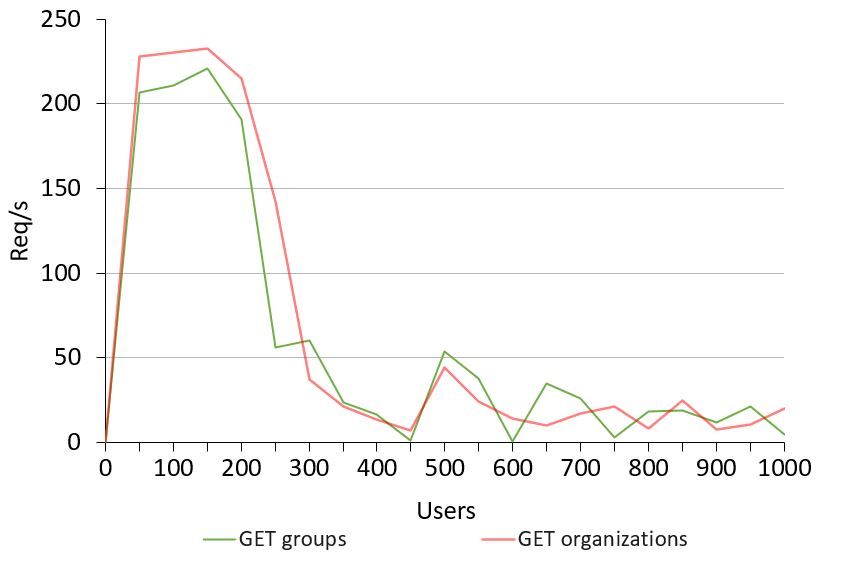
\includegraphics[width=.7\textwidth]{img/performance_evaluation/groups_organizations_individuais.JPG}
    \caption{\label{tab:throughput_groups_org}Throughput for group and organization requests}
  \end{figure}
  
  From the graphs in Figure \ref{tab:throughput_datasets} and \ref{tab:throughput_groups_org}, we can draw some conclusions:
  
  \begin{itemize}
      \item The requests per second increase up to 50 concurrent users, and remain without significant changes up to 200 users, which for now shows to be an interesting data to identify the limit of clients per server from which we will have finished the diminishing returns, and which would be the ideal number of clients to establish as a limit of clients per server. Furthermore, we can notice that the throughput of the requests to the set of groups and/or organisations is much higher, which lies in the fact that this data is much lighter;
      \item After the 200 user mark, there is a significant decrease in the system's ability to handle that many users, with the system's lower ability to manage the number of users suggesting a greater range in requests made per second, getting several inconsistent peaks. This happens most relevantly for requests to read datasets and resources, since the proportion of requests before and after the 200 users is not as noticeable as for organisations or groups;
      \item It would make sense for the throughput to be higher for reading a given resource compared to a given dataset, since its average response size is smaller than the latter. However, \textit{\gls{ckan}} forces the resource request to an extra computation, i.e., it accesses the dataset it belongs to and checks if it is in the dataset's resource list, if the resource is no longer present, then it is non-existent.
  \end{itemize}
  
  \begin{figure}[H]
    \centering
    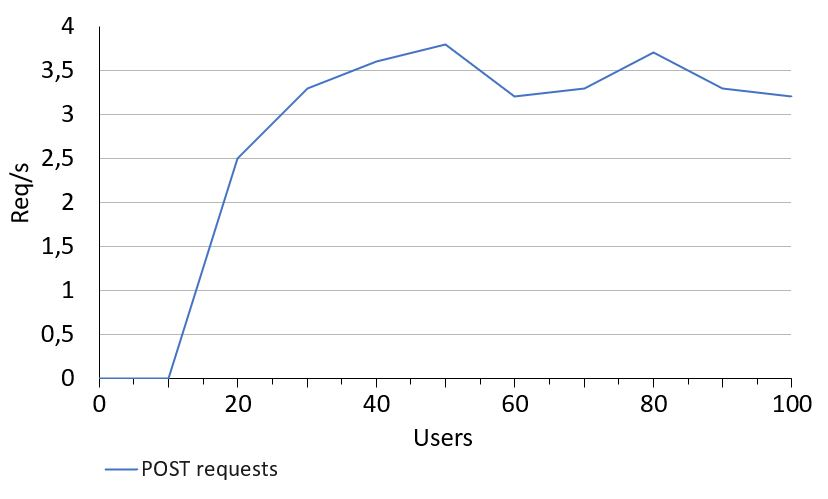
\includegraphics[width=.8\textwidth]{img/performance_evaluation/post_individual.JPG}
    \caption{\label{tab:throughput_write}Throughput for write requests}
  \end{figure}
  
  
  The graph in Figure \ref{tab:throughput_write} shows the huge demand for write requests, being the most relevant bottleneck in this set of requests. Note that the system does not allow to inserting more than one file (resource) at a time, which makes this process even more complex.
  
  
  \subsection{Response time}

  The second metric we sought to analyse was the time it takes the client to receive a response to a given request, distinguishing between each of the types and understanding what factors can influence this response time. As such, we present information in Table \ref{tab:time_individually}.
  
  We chose to analyse only the average time, since, for now, the average time allows us to draw the necessary conclusions for the elaboration of the tests in the following sections.
  
  \newpage
  
    \begin{table}[h]
    \centering
    \begin{tabular}{|>{\centering\arraybackslash}p{6.5cm}|>{\centering\arraybackslash}p{2.5cm}|>{\centering\arraybackslash}p{2cm}|>{\centering\arraybackslash}p{2.5cm}|>{\centering\arraybackslash}p{1cm}|} 
      \hline
      \textbf{Request} & \textbf{\# Requests} & \textbf{Average (ms)} & \textbf{Average size (bytes)} & \textbf{RPS} \\ 
      \hline
      GET /current\_package\_list\_with\_resources & 5178 & 12704 & 216203 & 19.5  \\ 
      \hline
      GET /package\_show?id & 7309 & 9891 & 10603 & 26.8   \\ 
      \hline
      GET /resource\_show?id & 7056 & 10459 & 772 & 25.0    \\
      \hline
      GET /organization\_list & 24350 & 3324 & 129 & 92.5   \\
      \hline
      GET /group\_list & 22222 & 3190 & 116 & 80.6   \\
      \hline
      POST requests & 179 & 9496  & 2178 & 3.5   \\ 
      \hline
    \end{tabular}
    \caption{\label{tab:time_individually}Individual Response Time }
  \end{table}
  
  Analysing Table \ref{tab:time_individually} we can draw three conclusions: 

  \begin{itemize}
    \item The average response time of the server to a given request depends mainly on the size of the response, that is, the smaller the size of the content we want to read, the faster the response will be (even suggesting that we are facing a logarithmic growth) and, consequently, the higher the throughput will also be;
    \item Although for the case of POST requests we consider a smaller sample, it manages to present an average response time almost equal to the reading of datasets with random id's in a sample with 10 times more users. This reinforces the impact that this type of request will have in a real scenario;
    \item The number of requests to the list of organisations is slightly higher than for groups, despite having a larger average size as a response, and we believe this is due to extra calculation that the latter performs, however, we cannot see where this actually happens.
  \end{itemize}
  
  
  \subsection{Summary}
  
  Finally, after these first tests, we can make an overall analysis and make some decisions for those that will follow:
  
  \begin{itemize}
      \item All clients are launched with the same process (running on a single core) by \textit{Locust}, which can end up being limiting when it comes to exploiting the maximum capacity of the available resources, and therefore also when it comes to getting a realistic sense of how the system works. Furthermore, all clients share the network bandwidth, which also limits the throughputs that we collect in these first attempts. However, even though we cannot do anything about the bandwidth sharing, when it comes to using only one core, we will try to exploit the load distribution feature \textit{Locust} has;
      \item Requests that require a random ID of a resource or dataset are time expensive compared to those that use a specific ID, and obviously in a real world scenario this would not happen, but for testing purposes the extra computation generating a random ID is needed. The system may have numerous resources and datasets and each with completely different sizes, so going the other way, such as a default ID, would be misleading; 
      \item In a realistic world scenario a user will not be making requests all the time with no break in between, so we will explore the wait between requests;
      \item \textit{\gls{ckan}} uses pagination when making datasets available to the user through the UI, as such it only loads x number of datasets (by default 20) which enables the insertion of a larger volume of data. We were able to reproduce the same pagination behavior in a similar way, and although we considered increasing the number of datasets in the system, we chose not to do so because as we can see from these early graphs, there is already a considerable amplitude difference between requests early on. However, due to paging, we believe that we could increase the number of data, with slight consequences up to 200 users and bigger problems thereafter. 
  \end{itemize}
    
    \section{Preliminary case}
    
        In this section, we will analyse the behavior of the system with the variety of all read requests and expose the system to the factors listed in the Section \ref{tab:request_factors}, i.e., waiting between requests, load distribution, and connection pool.
  
  
  \subsection{With variety}
  
  After in the previous section we understood how the system reacts if there is only one type of request being executed, in this section we will analyse its behavior if there are several types of requests being executed, more specifically, all the reading requests listed in Table \ref{tab:type_requests}. Furthermore, we will not consider any restrictions on the way requests are made, nor any changes in the way the system handles them, since the results of the tests in this section will be used as a comparison to the remaining ones in this performance evaluation.
  
  
  \subsubsection{Throughput}
  
  It is to be expected that the evaluation of this metric will only corroborate the conclusions drawn in individual testing, since the only change from that testing is the request variety.
  
    \begin{figure}[H]
    \centering
    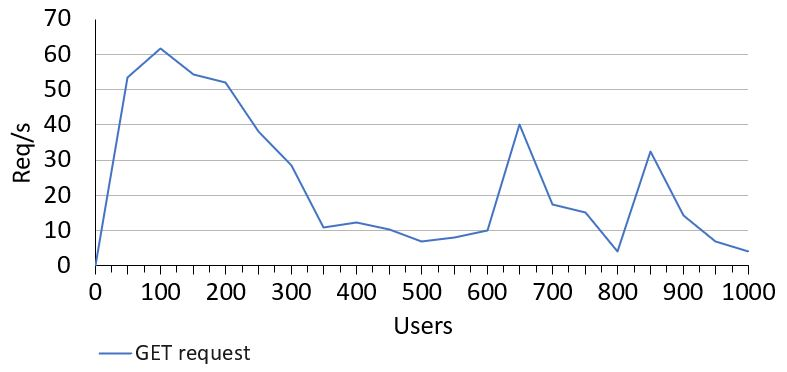
\includegraphics[width=.8\textwidth]{img/performance_evaluation/normal.JPG}
    \caption{\label{tab:throughput_normal}Throughput}
  \end{figure}
  
  We can then prove what we expected from the graph in Figure \ref{tab:throughput_normal}, that is, that the 200 users remains the point at which a significant drop in the number of requests executed per second begins to appear. Moreover, the large amplitude between requests exists from the 200 concurrent user mark onwards, with the same irregular peaks present in the individual case.
  
  Next, we present the table \ref{tab:geral_norma} with general information regarding the number of requests executed per second, as well as other information that may be useful for making comparisons with other tests.
  
  \newpage
  
  \begin{table}[h]
    \centering
    \begin{tabular}{|>{\centering\arraybackslash}p{2.5cm}|>{\centering\arraybackslash}p{2cm}|>{\centering\arraybackslash}p{4cm}|>{\centering\arraybackslash}p{1.5cm}|} 
      \hline
      \textbf{\# Requests} & \textbf{\# Fails} & \textbf{Average size (bytes)} & \textbf{RPS} \\ 
      \hline
      8096 & 355 & 50200 & 28.8  \\ 
      \hline
    \end{tabular}
    \caption{\label{tab:geral_norma}Request statistics}
  \end{table}
  
  Of the 8096 requests made to the system, 335 fail (note that this failure is not harmful to the system), that is, 335 exceed the timeout in terms of time for the server to respond to something, which is due to the higher traffic of requests, but we will address more clearly the occasions when this happens afterwards.
  
  \subsubsection{Response Time}
  
  For this metric, we will look at the median response time, i.e., the time value that separates the highest and lowest half of our sample of server response times to requests made to it, and the 95\% percentile, i.e., how long it takes the server to respond to requests 95 percent of the time. It is to be expected that from 200 users onwards, these values will start to increase with some significance, and that, as with throughput, there will also be a certain range between users and irregular peaks.
  
  \begin{figure}[H]
    \centering
    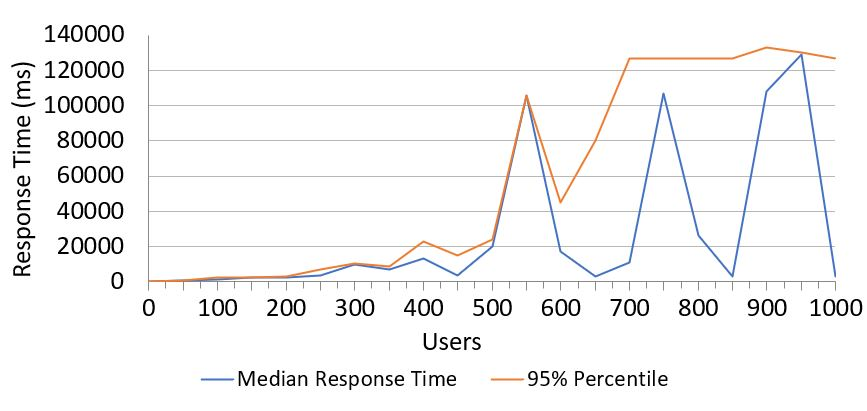
\includegraphics[width=1\textwidth]{img/performance_evaluation/normal_time.JPG}
    \caption{\label{tab:time_normal}Response Time}
  \end{figure}
  
  \newpage
  
  Looking at the graph in figure \ref{tab:time_normal}, we can then confirm the expected: 
  
  \begin{itemize}
      \item Until the 200 users mark the system responds in an acceptable way, more specifically, the server has a median of 2430 ms and 95\% of the time it can respond in a maximum of 3170 ms to the requests that are made to it. However, although we take into account that most of the requests are somewhat heavy, 3s is something that we believe we can improve;
      \item After 200 concurrent users, the system begins to behave somewhat unpredictably, however, always in an unbearable way. It is worth mentioning the 500 users mark, since from that point on, the system starts to suffer more aggressively, since it goes from being able to respond 95\% of the time in a maximum of 24000 ms to values higher than 100000s, that is, an increase of more than 400\%, which results in the growth of faults in the system, since the timeout used for read requests is 5s.
  \end{itemize}
  
 To add an interesting statistic to compare later, the average response time was 9156 ms.
  
  \subsubsection{CPU and Disk Utilisation}
  
  For this evaluation, with the help of the Linux iostat command, we will make an analysis of the percentage of CPU usage that occurred during the execution at the user level (i.e. application) and, when it comes to disk usage, we chose to compile the information (tps - number of transfers per second to the device,  kb\_read/s - amount of data read from the device, kb\_wrtn/s - amount of data written to the from the device) of the devices into one, these being sda, sdb and sdd, which were the ones that showed changes during the execution of the test. As far as the CPU is concerned, since we have 80 CPUs, the result is an average of the usage of each one.
  
  We provide the above information for 100, 500 and 1000 users in the Table \ref{tab:cpu_normal}, i.e. the CPU and disk utilisation from the initial moment up to 100 users, then the utilisation between 100 and 500 users, and finally between 500 and 1000.
 
  \newpage

\begin{table}[h!]
\centering
\begin{tabular}{|c|c|c|c|c|} 
\hline
\multirow{2}{*}{\textbf{Users }} & \multirow{2}{*}{\textbf{~\%CPU}} & \multicolumn{3}{c|}{\textbf{Devices}}                     \\ 
\cline{3-5}
                                 &                                  & \textbf{tps} & \textbf{kB\_read/s} & \textbf{kB\_wrtn/s}  \\ 
\hline
100  & 1,5 & 2,1  & 0  &  36,2                  \\ 
\hline
500  & 0,8 & 2,2 & 0 & 35,5                   \\ 
\hline
1000 & 0,6 & 2,3 & 0 & 27,8                 \\ 
\hline
\end{tabular}\caption{\label{tab:cpu_normal}CPU and Disk utilisation}
\end{table}


This way we realize that the fact that \textit{Locust} uses only one process results in almost zero CPU usage and, in turn, Disk usage is also residual. Note that both metrics are influenced, in a minimal way, by other processes than those used by the tests or the server. Furthermore, no information is read from the devices, since it is already in the CPU cache, loaded at the beginning of the test.
  
  
  \subsection{With variety and waiting between requests}
  
  At this point, let's evaluate the system taking into account that there are waits between requests. To do this, we changed our script by adding an attribute that \textit{Locust} provides for the User class, more specifically, wait\_time, which introduces a delay after the execution of each task.
    
  \begin{verbatim}
   wait_time = constant_throughput(0.25)
  \end{verbatim}
  
  The above assignment guarantees that each User runs a task 0.25 times per second, i.e., 1 task every 4 seconds, which seems to us a realistic estimate of system usage by a client on average.

  \subsubsection{Throughput}
  
  Something we can expect before testing this metric is that the initial growth of requests may not be as steep as for a no-wait test. As such, it should also have an influence on the speed with which the system will reach the optimal concurrency situation, more specifically, it should take longer to reach that state.

  \begin{figure}[H]
    \centering
    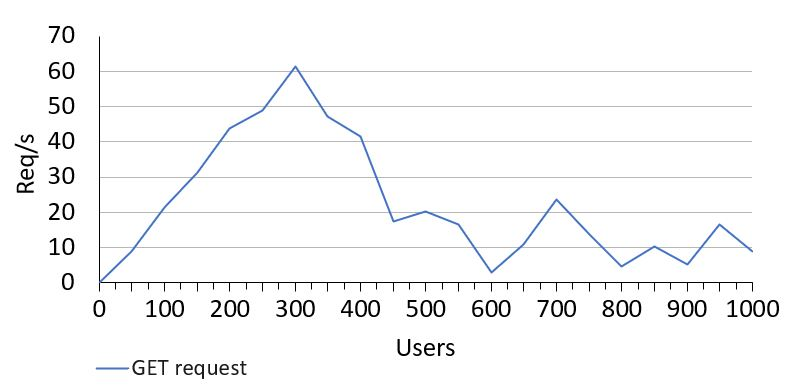
\includegraphics[width=.8\textwidth]{img/performance_evaluation/wait.JPG}
    \caption{\label{tab:thorughput_wait}Throughput with waiting between requests}
  \end{figure}
  
  From the Figure \ref{tab:thorughput_wait} we can conclude the following:
  
  \begin{itemize}
      \item The wait between requests causes what would be expected, that is, a less gradual growth until diminishing returns are reached, which in this case we can point to end up at 400 users. This is good news, since by considering a case closer to reality, we managed to double the ideal competition limit;
      \item Passing the mark of the ideal number of concurrent users, in contrast to the large range between requests when there is no wait, here the range, while still existing, exists to a lesser extent.
  \end{itemize}
  
  From the same test performed for the elaboration of the graph of the Figure \ref{tab:thorughput_wait}, we were able to extract information regarding the total values of the requests made, among other values. We present this information available in the following Table \ref{tab:geral_wait}.
  
  \begin{table}[h]
    \centering
    \begin{tabular}{|>{\centering\arraybackslash}p{2.5cm}|>{\centering\arraybackslash}p{2cm}|>{\centering\arraybackslash}p{4cm}|>{\centering\arraybackslash}p{1.5cm}|} 
      \hline
      \textbf{\# Requests} & \textbf{\# Fails} & \textbf{Average size (bytes)} & \textbf{RPS} \\ 
      \hline
      5967 & 237 & 51139 & 21.6  \\ 
      \hline
    \end{tabular}
    \caption{\label{tab:geral_wait}Request statistics with waiting between requests}
  \end{table}
  
   We then see that fewer requests are made in total relative to a system without waits, which makes perfect sense. Without wanting to fall into redundancy, more waiting, fewer requests, however, this is not something negative, just a consequence of the reality of a system in which all users are not constantly making requests.
  
  \subsubsection{Response Time}
  
  Now, we try to understand how the system performs in terms of time to process and respond to a request. We again expect that, just as happened with the throughput, the response times should start to increase later, less gradually.
  
  \begin{figure}[H]
    \centering
    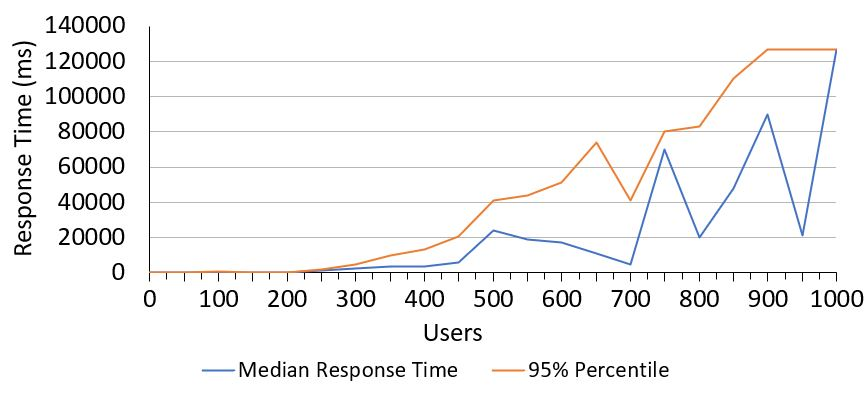
\includegraphics[width=1\textwidth]{img/performance_evaluation/wait_time.JPG}
    \caption{\label{tab:time_wait}Response time with waiting between requests}
  \end{figure}
  
  Thus, with the help of Figure \ref{tab:time_wait} we can confirm what we theorize. On the one hand, the 95\% percentile and the median start showing signs of increase even before 200 users in a system without waits between requests, and the 95\% percentile reaches the maximum value of 127000 ms at the 700 users mark. On the other hand, for the system we are considering in this subsection the median starts to increase considerably after 450 users, and the 95\% percentile start increasing after 300 users and reaches the maximum value at the 900 users mark. 
  From the same test, we also took the average response time, this was 10190 ms.
  
  \subsubsection{CPU and Disk Utilisation}
  
  We expect that, unlike the first scenario, there will be a greater CPU usage after 100 users, since until this mark the ideal number of concurrent users in the system has not yet been reached. Regarding the use of the Disk, we believe that it will again be residual.

\newpage

\begin{table}[h!]
\centering
\begin{tabular}{|c|c|c|c|c|} 
\hline
\multirow{2}{*}{\textbf{Users }} & \multirow{2}{*}{\textbf{~\%CPU}} & \multicolumn{3}{c|}{\textbf{Devices}}                     \\ 
\cline{3-5}
                                 &                                  & \textbf{tps} & \textbf{kB\_read/s} & \textbf{kB\_wrtn/s}  \\ 
\hline
100  & 0,5 & 3,2  & 0  &  34,4                   \\ 
\hline
500  & 1,1 & 2,5 & 0 & 33,5                    \\ 
\hline
1000 & 0,4 & 2,1 & 0 & 23,9                 \\ 
\hline
\end{tabular}\caption{\label{tab:cpu_waiting}CPU and Disk utilisation}
\end{table}

  We confirm the expected through Table \ref{tab:cpu_waiting}.
 

  \subsection{With variety, waiting between requests and distributed load}

  We now consider two factors, namely, the wait between requests, since it showed to be a factor to consider in a realistic case, and, additionally, the load distribution that \textit{Locust} allows.
  
  While a single process running Locust can simulate a significant number when it comes to throughput, for more complex or higher load tests, scaling to multiple processes, and even multiple machines, is something to strongly consider. In our case, since we have hardware with higher capacity than usual, we will explore this feature. To do so, we use the same script as in the previous section, we just modify the way we run it, as well as the number of instances created, that is, we run one instance of Locust in one terminal using the master flag and 40 other instances (we use 40 since, typically, the Locust team suggests using one worker instance per processor core) in different terminals using the worker flag. The master instance tells the workers when to stop or start and does not run Users, while the workers run Users and send back statistics to the master.
  
  \subsubsection{Throughput}
  
  For this metric, we think that the distribution load will result in better overall throughput, because the process cores will be less heavy than a single would be, and for that very reason, probably the moment of diminishing returns will last longer.
  
    \begin{figure}[H]
    \centering
    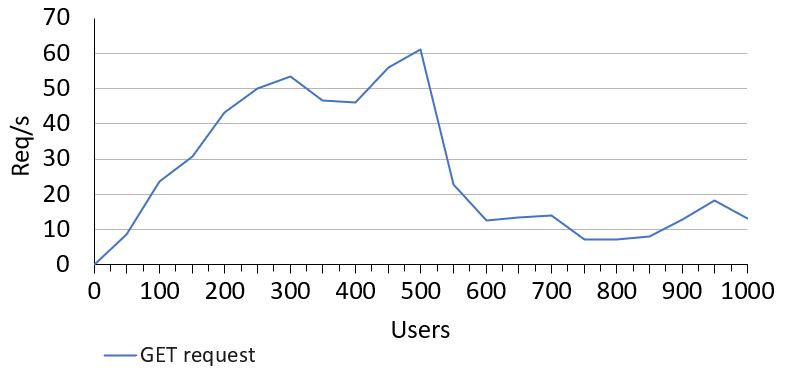
\includegraphics[width=.8\textwidth]{img/performance_evaluation/distributed.JPG}
    \caption{\label{tab:throughput_dist_load}Throughput with waiting between requests and distributed load}
  \end{figure}
  
  Analysing Figure \ref{tab:throughput_dist_load} we conclude that: 
  
  \begin{itemize}
      \item Our predictions were true, that is, the moment of diminishing returns lasts a little longer, from 200 (as in the test of waits between requests) to 500 concurrent users, which is a record number within the tests we ran;
      \item Similar to the test in the previous section, the range is smaller than the initial tests due to the wait, which allows to have fewer peaks.
  \end{itemize}

  More general statistics regarding the response to requests are presented below in Table \ref{tab:geral_dist_load}.
  
  \begin{table}[h]
    \centering
    \begin{tabular}{|>{\centering\arraybackslash}p{2.5cm}|>{\centering\arraybackslash}p{2cm}|>{\centering\arraybackslash}p{4cm}|>{\centering\arraybackslash}p{1.5cm}|} 
      \hline
      \textbf{\# Requests} & \textbf{\# Fails} & \textbf{Average size (bytes)} & \textbf{RPS} \\ 
      \hline
      8342 & 68 & 54369 & 29.4  \\ 
      \hline
    \end{tabular}
    \caption{\label{tab:geral_dist_load}Request statistics with waiting between requests and distributed load}
  \end{table}
  
  So we broke another record, this time for the total number of requests answered, although it is residual. On the contrary, we managed to decrease the number of failures, which is the result of an improved system capacity, and now, in the analysis of response times, we will understand why.
  
  \subsubsection{Response Time}
  
  In the analysis of this metric we expect to see a lower median response time, and consequently fewer peaks relative to the previous tests due to the removal of the overhead from one process, spreading it across multiples. Also, for the 95\% percentile, we expect that it will not reach stabilization, since it would take more users for that moment to happen.
  
  \begin{figure}[H]
    \centering
    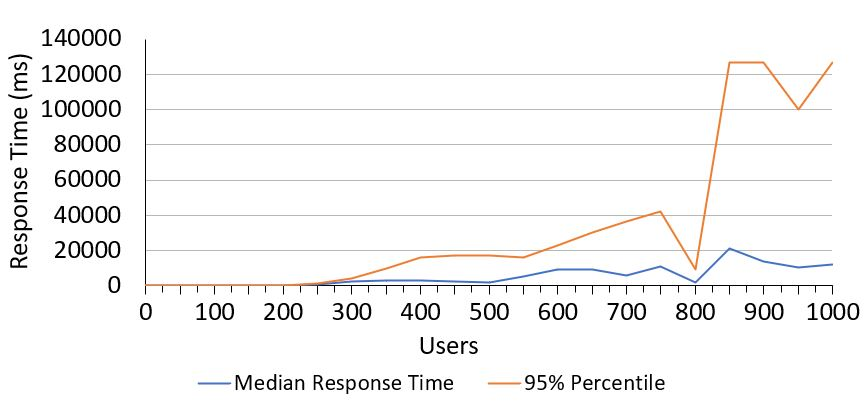
\includegraphics[width=1\textwidth]{img/performance_evaluation/distributed_time.JPG}
    \caption{Response time with waiting between requests and distributed load}
  \end{figure}
  
  Observing the graph in the figure above, we draw the following conclusions:
  
  \begin{itemize}
      \item The median remained until 1000 users without significant variations in its amplitude compared to the other tests, nor did we detect any peak of relevance. In addition, we can observe that the median, as for the previous situations, started to increase with greater intensity from the ideal number of concurrent users (500), this makes sense, since a lower ability to deal with concurrency results in a longer time to respond to requests;
      \item The fact that the median is below 5000s more than half the time explains the low number of failed requests, which is also positive to draw from this metric;
      \item For the 95\% percentile, we can confirm that it effectively does not stabilize at any maximum, and so we can say with certainty that it would take a few more users for this to happen.
  \end{itemize}
  
  We also took the average response time from the same test, this was 5684 ms.
  
  \subsubsection{CPU and Disk Utilisation}
  
  We anticipate that the load distribution will increase CPU usage in percentage, however, we are unable to predict how much the increase will be. Furthermore, we believe that Disk usage will again be residual. We present the relative information in the Table \ref{tab:cpu_dist}.


\begin{table}[h!]
\centering
\begin{tabular}{|c|c|c|c|c|} 
\hline
\multirow{2}{*}{\textbf{Users }} & \multirow{2}{*}{\textbf{~\%CPU}} & \multicolumn{3}{c|}{\textbf{Devices}}                     \\ 
\cline{3-5}
                                 &                                  & \textbf{tps} & \textbf{kB\_read/s} & \textbf{kB\_wrtn/s}  \\ 
\hline
100  & 9,8 & 3,1  & 0  &  32,7                   \\ 
\hline
500  & 10,2 & 2,3 & 0 & 46,2                    \\ 
\hline
1000 & 8,6 & 1,9 & 0 & 35,5                 \\ 
\hline
\end{tabular}\caption{\label{tab:cpu_dist}CPU and Disk utilisation}
\end{table}

  For this scenario, we also ran the Linux top command to get a sense of the CPU utilisation of each processor involved in the testing, and realised that on average each processor was using 20\% of its capacity.

  The CPU utilisation increases about 10 times, which we can explain by the following: each processor uses on average one fifth of its capacity, and since we use 40 processors in the load distribution, which corresponds to half of the possible CPUs, that is, 50\% of the maximum machine capacity, then we conclude that on average the total usage should be:
  
  \begin{verbatim}
      %CPU = (0,2 * 0,5) * 100 % = 10 %
  \end{verbatim}
  
  \subsection{With variety, waiting between requests, distributed load and connection pool}
  
  In addition to the factors considered earlier in this section, we will now add a connection pool, a configuration enabled by \textit{\gls{ckan}}, which uses \textit{SQLAlchemy} (a \textit{Python} \textit{SQL} toolkit and Object Relational Mapper that gives application developers the full power and flexibility of \textit{SQL}) to take advantage of this.
  
  The connection pool technique is used to keep long-running connections in memory for efficient reuse. In addition, it provides management of the total number of connections that the system must use concurrently. To do this we had to add to our \textit{\gls{ckan}} configuration file:
  
  \begin{verbatim}
   sqlalchemy.pool_size = 40
   sqlalchemy.max_overflow = 20
  \end{verbatim}
  
  So we have a pool with size 40, i.e. the number of core processors in our machine, and we allow 20 more connections to be used if necessary, which gives a total of 60 connections, and does not jeopardize the full utilisation of our hardware.
  
  \subsubsection{Throughput}
  
  Regarding this metric, we expect similar behavior to the previous case, but that the better management by the connection pool may be visible at some point in the test.
  
  \begin{figure}[H]
    \centering
    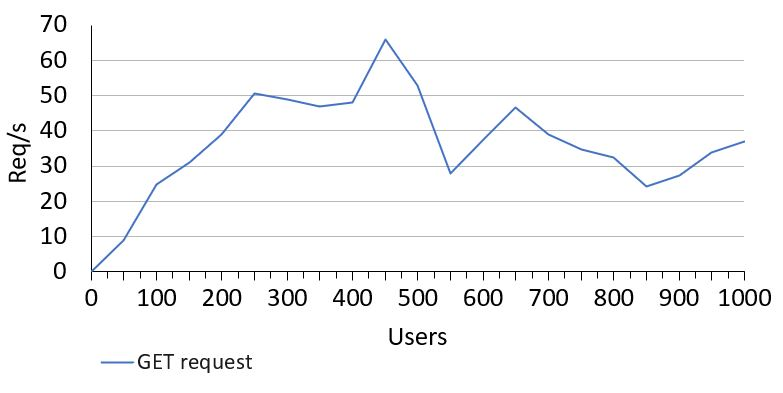
\includegraphics[width=.8\textwidth]{img/performance_evaluation/pool.JPG}
    \caption{Throughput with waiting between requests, distributed load and connection pool}
  \end{figure}
  
  Thus, we confirmed that the system behaves in a similar way, but that after 500 users, which remains as the final moment of diminishing returns, it manages to maintain a throughput between 25 and 45 requests per second until the final moment of the test. This proves the efficiency of the pool management.
  
In order to get a general overview of this test, we can see more information about it in the Table \ref{tab:geral_pool}.

\newpage
  
    \begin{table}[h]
    \centering
    \begin{tabular}{|>{\centering\arraybackslash}p{2.5cm}|>{\centering\arraybackslash}p{2cm}|>{\centering\arraybackslash}p{4cm}|>{\centering\arraybackslash}p{1.5cm}|} 
      \hline
      \textbf{\# Requests} & \textbf{\# Fails} & \textbf{Average size (bytes)} & \textbf{RPS} \\ 
      \hline
      9545 & 71 & 52278 & 35.0  \\ 
      \hline
    \end{tabular}
    \caption{\label{tab:geral_pool}Request statistics with waiting between requests, distributed load and connection pool}
  \end{table}
  
  As we can see, the better management carried out by the connection pool allowed the total number of requests to increase slightly.
  
  \subsubsection{Response Time }
  
  In Figure \ref{tab:pool_time} we will see a graph of the response times for the latter case. At the outset, after improving the throughput, we believe that the response time will also show better results, leveraged by the efficient use of connections.
  
  \begin{figure}[H]
    \centering
    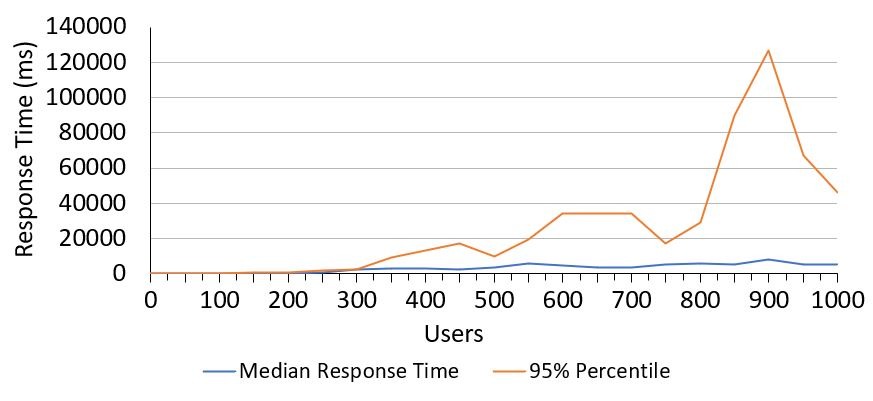
\includegraphics[width=1\textwidth]{img/performance_evaluation/pool_time.JPG}
    \caption{\label{tab:pool_time}Response time with waiting between requests, distributed load and connection pool}
  \end{figure}
  
  Viewing the graph above, we then know that, for the first time, we get a system that can reach 1000 users without ever getting a median greater than 10000ms, demonstrating an almost flat line from start to finish. Certainly, this system can handle an even larger number of users. However, there is no point in exploring further, since it is already unthinkable to even consider requests with a response of about 10s.
  
  As for the average response time, this was 5785 ms.
  
  \subsubsection{CPU and Disk Utilisation}
  
  CPU and Disk usage should be similar to the previous scenario, with a slight difference in CPU usage, which should be more balanced due to the connection pool. The information is presented below in table \ref{tab:cpu_load}.

\begin{table}[h!]
\centering
\begin{tabular}{|c|c|c|c|c|} 
\hline
\multirow{2}{*}{\textbf{Users }} & \multirow{2}{*}{\textbf{~\%CPU}} & \multicolumn{3}{c|}{\textbf{Devices}}                     \\ 
\cline{3-5}
                                 &                                  & \textbf{tps} & \textbf{kB\_read/s} & \textbf{kB\_wrtn/s}  \\ 
\hline
100  & 9,2 & 5,9  & 0  & 65,4                   \\ 
\hline
500  & 10,0 & 2,91 & 0 & 49,3                    \\ 
\hline
1000 & 9,3 & 2,0 & 0 & 38,2                 \\ 
\hline
\end{tabular}\caption{\label{tab:cpu_load}CPU and Disk utilisation}
\end{table}

  We verified what we had predicted, however, the values corresponding to the transfers per second up to 100 users, as well as the number of kB written cause some surprise, and we do not know exactly what caused this increase in relation to the previous scenario.

  \subsection{Summary}
  
  After all the tests of the preliminary case are completed, we compare the former with the latter:
  
  \begin{itemize}
      \item 22 \% gain in the total number of requests executed;
      \item The average response time was almost halved (down about 40\%), which turned out to be the biggest gain;
      \item Decrease of 80\% in the number of failed requests.
  \end{itemize}
  
  We can then state that we have achieved a more efficient system than the one we initially predicted. However, we emphasize that these tests are a pessimistic estimation of how our system will work, mainly due to bandwidth sharing and write requests. We look at this pessimistic estimation as a positive thing, since in a real scenario our system will be able to give an even better answer than the one we presented.
  
  Finally, we conclude that in the realistic scenario that we will present next it will make sense to approach a system like the last one we tested, i.e. with waits between orders, load distribution and connection pool, since they proved to be closer to reality and allowed a better use of the resources we had available.

    
    \section{Realistic Case}
    
        
  
  This section includes the analysis and evaluation of the realistic case, that is, the case where both reading and writing requests are possible, with their respective probabilities of occurrence listed in table \ref{tab:type_requests}. In addition, we considered the waiting between requests, load distribution and connection pool, as we just mentioned in the last section.

  We believe it would be best to do an analysis of how each request influenced the big picture, before evaluating metrics regarding throughput and response time. As such, we present Table \ref{tab:geral_real} on the next page.
  
\begin{sidewaystable}[h!]
    \centering
    \begin{tabular}{|l|l|l|l|l|l|}
      \hline
      \textbf{Request} & \textbf{\# Requests} & \textbf{\# Fails} & \textbf{Average (ms)} & \textbf{Average size (bytes)} & \textbf{RPS} \\ 
      \hline
      GET /current\_package\_list\_with\_resources & 756 & 55 & 17890 & 369734 & 3.0    \\ 
      \hline
      GET /resource\_show?id & 626 & 38 & 16830 & 763 & 2.5   \\ 
      \hline
      GET /package\_show?id & 799 & 32 & 14279 & 10652 & 3.2    \\
      \hline
      GET /organization\_list & 481 & 25 & 15864 & 124 & 1.9   \\
      \hline
      GET /group\_list & 473 & 19 & 13284 & 113 & 1.9   \\
      \hline
      POST /package\_create & 163 & 118 & 18232 & 1063 & 0.7   \\ 
      \hline
      POST /package\_revise & 138 & 16 & 23257 & 4577 & 0.6   \\ 
      \hline
      POST /resource\_create\_default\_resource\_views & 109 & 5 & 12272 & 332 & 0.4   \\ 
      \hline
      POST /datastore\_create & 101 & 5 & 15491 & 106 & 0.4    \\
      \hline
      Aggregated & 3646 & 313 & 16166 & 79395 & 14.5   \\ 
      \hline
    \end{tabular}
    \caption{\label{tab:geral_real}Request statistics for reading and writing requests}
\end{sidewaystable}
    \clearpage% Flush page

  
  As we can already see, the two biggest times are the two for writing requests, and so we already have an idea of how influential these are going to be in the big picture. Also, the number of total requests, as we can see, is the lowest so far, which was also to be expected.
    
  \subsection{Throughput}
  
  For this metric, we already know that adding write requests will have impact on the number of requests executed per second.
  
  \begin{figure}[H]
    \centering
    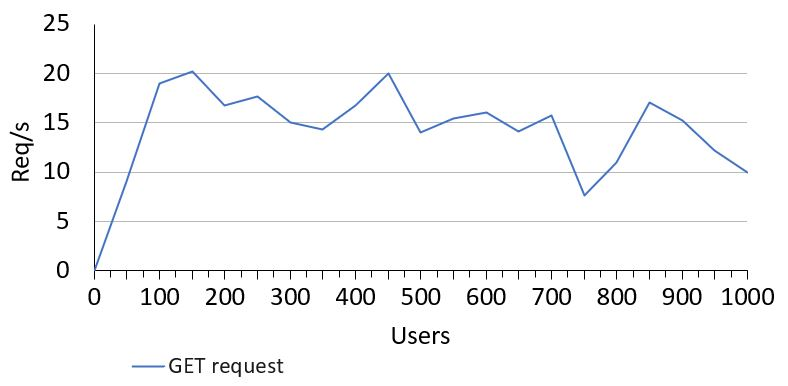
\includegraphics[width=.8\textwidth]{img/performance_evaluation/real.JPG}
    \caption{\label{tab:throughput_real}Throughput for reading and writing requests}
  \end{figure}
  
  We can then conclude from the Figure \ref{tab:throughput_real} the following: 
  
  \begin{itemize}
      \item There is a certain balance in the values from start to finish, which highlights the factors considered (without them, we would certainly have to reduce the sample of users);
      \item The 100-user mark proves to be the optimal number of concurrency, since in addition to reaching the maximum peak of 19 requests per second, we consider that a user would make 1 request every 4 seconds, which making the proportion, 100 users would make a total of 25 req/s, which being a bit higher than the 19 req/s would have a slight affect at the level of response time.
  \end{itemize}. 
  
  
  \subsection{Response time}
  
  For response time, we also expect the worst result so far. Nevertheless, we expect that the median response time variation, like throughput, will not show a considerable range between users.
  
  \begin{figure}[H]
    \centering
    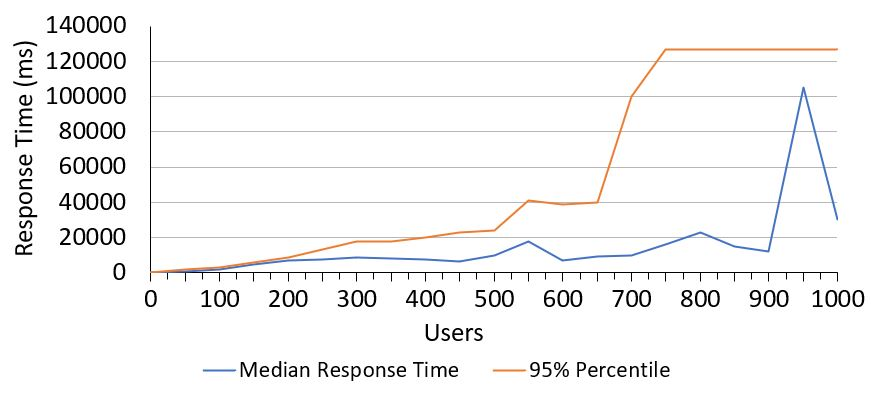
\includegraphics[width=1\textwidth]{img/performance_evaluation/real_time.JPG}
    \caption{\label{tab:time_real}Response time for reading and writing requests}
  \end{figure}
  
  Figure \ref{tab:time_real} tells us that:
  
  \begin{itemize}
      \item In fact, the variation of the median is not as considerable as in most of the cases already worked on, although its sharpest rise starts earlier, from the 50 users, which registers a 420 ms mark as far as the median is concerned, while the 100 users that we had referenced as the competition ideal, registers 1900 ms;
      \item The 95\% percentile ends up showing a balanced growth without peaks until it reaches a maximum peak of 127000 ms at 750 users and then stabilises.
  \end{itemize}
  
\newpage  
  
  \subsubsection{CPU and Disk Utilisation}
  
  In a realistic scenario, we believe that the CPU utilisation will be the same as obtained from the scenarios with load distribution and that the Disk utilisation will show a marked difference from what we have analysed so far, due to the write requests. To scrutinise what we have stated, we present the Table \ref{tab:cpu_real}.

\begin{table}[h!]
\centering
\begin{tabular}{|c|c|c|c|c|} 
\hline
\multirow{2}{*}{\textbf{Users }} & \multirow{2}{*}{\textbf{~\%CPU}} & \multicolumn{3}{c|}{\textbf{Devices}}                     \\ 
\cline{3-5}
                                 &                                  & \textbf{tps} & \textbf{kB\_read/s} & \textbf{kB\_wrtn/s}  \\ 
\hline
100  & 10,0 & 111,8  & 0,2  &  3814,8                   \\ 
\hline
500  & 10,1 & 151,7 & 0,5 & 8023,8                    \\ 
\hline
1000 & 9,5 & 90,5 & 0,4 & 4743,1                 \\ 
\hline
\end{tabular}\caption{\label{tab:cpu_real}CPU and Disk utilisation}
\end{table}

Thus, we conclude that what we predicted actually happens. The number of kB written per second increases considerably due to the existence of write requests on the devices, which consequently causes differences in the total data present in the system, and so when read requests are made, it is necessary to access the disk to access the new data, which are not yet in RAM and then in the CPU cache.

  
  \subsection{Summary}
  
  We conclude this section with a positive balance. Based on what we have just examined, we can consider that the ideal number of users of our system would be 100 users and would serve for research teams from an institute like \gls{inesctec} to work on the platform. However, recognizing the pessimistic estimate we have, we are confident that in a real world scenario our system could possibly handle far more users, as well as enjoying an improvement of the available resources.
  

\chapter{Conclusions}

    \label{ref:chapter_5}

This final chapter summarizes the main contributions of this dissertation and discusses guidelines for future work.

The work reported in this dissertation addressed the viability of using \gls{sdms}s in the daily life of scientific communities, proposing \textit{\gls{ckan}} as the best solution at the moment. However, we cannot deny that  \textit{\gls{eudat}} is an extremely interesting system and that if one day it is made available for local development it may become a more attractive solution than  \textit{\gls{ckan}}.

The solution produced led to the conclusion that it will be difficult to achieve a universal system that can meet the needs of all scientific institutions or individual researchers. Moreover, the \gls{sdms}s themselves do not appear to be seeking convergence towards universal use \citep{assante}, but we should emphasize that \textit{\gls{eudat}} has the greatest potential to achieve this. As far as the \gls{sail} project is concerned, we are confident that the system based on  \textit{\gls{ckan}} has been able to meet its requirements, in general.

The benchmarking performed showed promising results, and taking into account that our estimation is pessimistic, we believe that the system could respond even better in a real context. Nevertheless, it should be kept in mind that due to the hardware available for testing, we can only extrapolate its usability.

The final conclusion is that the future of research will increasingly depend on these systems, and on how, above all, they will manage to convince the entire scientific community to come on board \citep{poschen}. This will require robust documentation of the systems and developer communities ready to help \citep{vardigan}, as the biggest barrier remains a certain need for technical expertise to exploit the full potential of the technologies \citep{9}.

\section{Future work}

One of the major goals of this dissertation was to recreate the system in an \gls{hpc} environment with the help of an infrastructure such as \gls{macc}. As such, it would be worth exploring this possibility while keeping in mind the guidelines set out. In particular, it would also be interesting to consider for the \gls{macc} other hypotheses beyond the produced system, such as the possible insertion of Deucalion in the  \textit{\gls{eudat}} network,  which would allow customisation and full control of its services.

 \textit{\gls{ckan}} is very close to presenting its new version 2.10. Although we don't know to what extent it may affect the functionality of this system, we have the expectation that it may bring more quality and potential to its use. In addition, it will allow the stability of certain extensions, which is not possible with the current (not stable) master version. In the future, there are two main features that we suggest to be integrated into the system that are not planned for the new version: upload/delete of multiple files and statistics regarding the use of the datasets, such as qualitative evaluation and number of file downloads.

Finally, the strongest suggestion for future work is to turn the software that has been developed into production and explore its functionality in a real-world context. Ideally, it would be interesting to use the system in the service of a research institution like \gls{inesctec} or HASLab.


    \bibliographystyle{plainnat}
    \bibliography{dissertation}
\end{document}
